\section{ỨNG DỤNG HÌNH HỌC CỦA TÍCH PHÂN}
\subsection{LÝ THUYẾT CẦN NHỚ}
\subsubsection{Diện tích hình phẳng giới hạn bởi đồ thị $y=f(x)$, trục hoành và hai đường thẳng $x=a$, $x=b$\quad $(a<b)$.}
\begin{enumerate}[\iconMT]
	\item \indam{Công thức tính:}\\
	\begin{minipage}[b]{6cm}
		\boxmini{$S_{(H)}=\displaystyle \int\limits_{a}^{b} \big|f(x)\big|\mathrm{\,d}x$}
		\vspace{1.5cm}
	\end{minipage}\hspace{1cm}
	\begin{minipage}[b]{9cm}
		\begin{khung4}{Lưu ý}
			\begin{itemize}
				\item [\iconCH] Nếu $f(x)$ không đổi dấu trên $[a;b]$ thì $$\displaystyle \int\limits_{a}^{b} \big|f(x)\big|\mathrm{\,d}x=\bigg|\displaystyle \int\limits_{a}^{b} f(x)\mathrm{\,d}x\bigg|.$$
				\item [\iconCH] Nếu đề chưa cho (\textit{hoặc thiếu}) cận, thì ta giải phương trình $f(x)=0$ để tìm cận.
			\end{itemize}
		\end{khung4}
	\end{minipage}
	\item \indam{Minh họa hình ảnh:}\\
	\hspace*{1cm}\begin{tikzpicture}[smooth,samples=300,scale=1.2,>=stealth,font=\footnotesize]
		\draw[->] (-0.8,0)--(4.5,0) node[below]{$x$};
		\draw[->] (0,-0.5)--(0,3) node[right]{$y$};
		\draw (0,0) node[below left]{$O$};
		\draw[blue,line width=0.7pt,domain=0.3:3.2] plot(\x,{0.3*(\x-1)^2+1})node[above right]{\scriptsize $y=f(x)$};
		\draw[fill=black] (1,0) circle(1pt) (3,0) circle(1pt);
		\draw[dashed] (1,0)node[below]{$a$}--(1,1) (3,0)node[below]{$b$}--(3,2.2);
		\fill[pattern=north west lines] (1,0)--plot[domain=1:3](\x,{0.3*(\x-1)^2+1})--(3,0)--cycle;
		\draw[->] (2.5,0.5)--(3.7,1) node[right]{$S$};
		\node[right] at (-1,-2.2) {\fbox{$S=\displaystyle \int\limits_{a}^{b} \big|f(x)\big|\mathrm{\,d}x=\displaystyle \int\limits_{a}^{b} f(x)\mathrm{\,d}x$}};
	\end{tikzpicture}
	\hspace{1cm}
	\begin{tikzpicture}[smooth,samples=300,scale=1.3,x=1.1cm,>=stealth,font=\footnotesize]
		\draw[->] (-0.8,0)--(3.5,0) node[below]{$x$};
		\draw[->] (0,-1)--(0,2) node[right]{$y$};
		\draw (0,0) node[below left]{$O$};
		\draw[blue,line width=0.7pt,domain=0.3:2.8] plot(\x,{(\x)*(\x-1.5)*(\x-2.5)})node[above right]{\scriptsize $y=f(x)$};
		\draw[fill=black] (0.5,0) circle(1pt) (1.5,0) circle(1pt) (2,0) circle(1pt);
		\draw[dashed] (0.5,0)node[below]{$a$}--(0.5,1) (2,0)node[above]{$b$}--(2,-0.5);
		\fill[pattern=north east lines] (0.5,0)--plot[domain=0.5:2](\x,{(\x)*(\x-1.5)*(\x-2.5)})--(2,0)--cycle;
		\node[right] at (-1,-2.2) {\fbox{$S=\displaystyle \int\limits_{a}^{b} \big|f(x)\big|\mathrm{\,d}x=\displaystyle \int\limits_{a}^{c} f(x)\mathrm{\,d}x-\displaystyle \int\limits_{c}^{b} f(x)\mathrm{\,d}x$}};
		\node[below] at (1.5,0) {$c$};
	\end{tikzpicture}
\end{enumerate}

\subsubsection{Diện tích hình phẳng giới hạn bởi đồ thị $y=f(x)$, $y=g(x)$ và hai đường thẳng $x=a$, $x=b$\quad $(a<b)$.}
\begin{enumerate}[\iconMT]
	\item \indam{Công thức tính:}\\
	\begin{minipage}[b]{6cm}
		\boxmini{$S_{(H)}=\displaystyle \int\limits_{a}^{b} \bigg|f(x)-g(x)\bigg|\mathrm{\,d}x.$}
		\vspace{1.5cm}
	\end{minipage}\hspace{1cm}
	\begin{minipage}[b]{9cm}
		\begin{khung4}{Lưu ý}
			\begin{itemize}
				\item [\iconCH] Nếu $f(x)-g(x)$ không đổi dấu trên $[a;b]$ thì $$\displaystyle \int\limits_{a}^{b} \big|f(x)-g(x)\big|\mathrm{\,d}x=\bigg|\displaystyle \int\limits_{a}^{b} (f(x)-g(x))\mathrm{\,d}x\bigg|.$$
				\item [\iconCH] Nếu đề chưa cho (\textit{hoặc thiếu}) cận, thì ta giải phương trình $f(x)=g(x)$ để tìm cận.
			\end{itemize}
		\end{khung4}
	\end{minipage}
	\item \indam{Minh họa hình ảnh:}\\
	\hspace*{1cm}\begin{tikzpicture}[smooth,samples=300,scale=0.8,>=stealth,font=\footnotesize]
		\draw[->] (-0.8,0)--(5.5,0) node[below]{$x$};
		\draw[->] (0,-0.5)--(0,3) node[right]{$y$};
		\draw (0,0) node[below left]{$O$};
		\draw[blue,line width=0.7pt,domain=0.3:3.2] plot(\x,{0.3*(\x-1)^2+1.5})node[right]{\scriptsize $y=f(x)$};
		\draw[magenta,line width=0.7pt,domain=0.3:3.4] plot(\x,{0.3*(\x-1.5)^2+0.5})node[below right]{\scriptsize $y=g(x)$};
		\draw[fill=black] (1,0) circle(1pt) (3,0) circle(1pt);
		\draw[dashed] (1,0)node[below]{$a$}--(1,1.5) (3,0)node[below]{$b$}--(3,2.7);
		\fill[pattern=north west lines,smooth] plot[domain=1:3](\x,{0.3*(\x-1)^2+1.5})--(3,1.175)--plot[domain=3:1](\x,{0.3*(\x-1.5)^2+0.5});
		\draw[->] (2.2,1.5)--(1.6,2.5) node[above]{$S$};
		\node[right] at (-0.8,-2) {\fbox{$S=\displaystyle \int\limits_{a}^{b} \bigg[f(x)-g(x)\bigg]\mathrm{\,d}x$}};
	\end{tikzpicture}
	\hspace{2cm}
	\begin{tikzpicture}[smooth,samples=300,scale=0.8,y=0.8cm,>=stealth,font=\footnotesize]
		\draw[->] (-0.8,0)--(7,0) node[below]{$x$};
		\draw[->] (0,-0.5)--(0,5) node[right]{$y$};
		\draw (0,0) node[below left]{$O$};
		\draw[blue,line width=0.7pt,domain=0.7:5.3] plot(\x,{0.5*(\x-1)*(\x-3)*(\x-5)+3})node[above right]{\scriptsize $y=f(x)$};
		\draw[magenta,line width=0.7pt,domain=0.5:5.3] plot(\x,{0.5*(\x-3)^2+1})node[below right]{\scriptsize $y=g(x)$};
		\draw[fill=blue] (1,0) circle(1pt) (4,0) circle(1pt) (5,0) circle(1pt)
		(1,3) circle(1.5pt) (4,1.5) circle(1.5pt) (5,3) circle(1.5pt);
		\draw[dashed] (1,0)node[below]{$a$}--(1,3)
		(4,0)node[below]{$c$}--(4,1.5)
		(5,0)node[below]{$b$}--(5,3);
		\fill[pattern=north west lines] (1,5)--plot[domain=1:5](\x,{0.5*(\x-3)^2+1})--(5,3)--plot[domain=5:1](\x,{0.5*(\x-1)*(\x-3)*(\x-5)+3})--cycle;
		\node[right] at (-0.8,-2.4) {\fbox{$S=\displaystyle \int\limits_{a}^{c} \bigg[f(x)-g(x)\bigg]\mathrm{\,d}x+\displaystyle \int\limits_{c}^{b} \bigg[g(x)-f(x)\bigg]\mathrm{\,d}x$}};
	\end{tikzpicture}
\end{enumerate}

\subsubsection{Tính thể tích của vật thể giới hạn bởi hai mặt phẳng $x=a$, $x=b$.}
\immini{Cho $T$ là một vật thể nằm giới hạn bởi hai mặt phẳng $x=a$ và $x=b$ (hình vẽ). Gọi $S(x)$ là diện tích thiết diện của vật thể cắt bởi mặt phẳng vuông góc với trục hoành tại điểm có hoành độ $x$, $(a \le x \le b)$.	Giả sử $S(x)$ là một hàm liên tục. Khi đó thể tích của vật thể $T$ được tính theo công thức
	\begin{center}
		\boxmini{$V=\displaystyle\int\limits_a^bS(x) \mathrm{\,d}x$}
	\end{center}
}{\hspace{0.5cm}
	\begin{tikzpicture}[>=stealth, scale=0.8]
		\draw plot[smooth,tension=.65] coordinates{(1,2) (2.5,2.3) (3.5,2.2)};
		\draw[dashed] plot[smooth,tension=.65] coordinates{(3.5,2.2) (4,2)};
		\draw plot[smooth,tension=.65] coordinates{(4,2) (5,2.2) (5.5,2.1)};
		\draw[dashed] plot[smooth,tension=.65] coordinates{(5.5,2.1) (6,2)};
		\draw plot[smooth,tension=.65] coordinates{(1,1) (2.3,0.5) (3.5,0.8)};
		\draw[dashed] plot[smooth,tension=.65] coordinates{(3.5,0.8) (4,1)};
		\draw plot[smooth,tension=.65] coordinates{(4,1) (5,0.7) (5.5,0.8)};
		\draw[dashed] plot[smooth,tension=.65] coordinates{(5.5,0.8) (6,1)};
		\draw[dashed] (1,1) arc (-90:90:.2 and 0.5);
		\draw (1,2) arc (90:270:.2 and 0.5);
		\draw[dashed] (4,1) arc (-90:90:.2 and 0.5);
		\draw (4,2) arc (90:270:.2 and 0.5);
		\draw (6,1) arc (-90:270:.2 and 0.5);
		\fill[pattern=north east lines] (4,1) arc (-90:90:.2 and 0.5)--(4,2) arc (90:270:.2 and 0.5)--cycle;
		\draw (-.5,0)--(0.5,0) (1,0)--(3.5,0) (4,0)--(5.5,0);
		\draw[dashed] (0.5,0)--(1,0) (3.5,0)--(4,0) (5.5,0)--(6,0);
		\draw[->] (6,0)--(7,0)node[below]{$x$};
		\draw (0.5,-1)--(0.5,3)--(1.5,3.5)--(1.5,2.2) (1.5,.8)--(1.5,-0.5)--(0.5,-1);
		\draw[dashed](1.5,2.2)--(1.5,.8);
		\draw[dashed] (1,1)--(1,0)node[below]{$a$};
		\coordinate (A) at (0.5,3);
		\coordinate (B) at (1.5,3.5);
		\coordinate (C) at (1.5,2.2);
		\tkzMarkAngle[size=.6](A,B,C);
		\draw (1.3,3.2) node {\footnotesize $P$};
		\draw (3.5,-1)--(3.5,3)--(4.5,3.5)--(4.5,2) (4.5,1)--(4.5,-0.5)--(3.5,-1);
		\draw[dashed](4.5,2)--(4.5,1);
		\draw[dashed] (4,1)--(4,0)node[below]{$x$};
		\coordinate (D) at (3.5,3);
		\coordinate (E) at (4.5,3.5);
		\coordinate (F) at (4.5,2);
		\tkzMarkAngle[size=.6](D,E,F);
		\draw (4.3,3.2) node {\footnotesize $R$};
		\draw (5.5,-1)--(5.5,3)--(6.5,3.5)--(6.5,-0.5)--(5.5,-1);
		\draw[dashed] (6,1)--(6,0)node[below]{$b$};
		\coordinate (G) at (5.5,3);
		\coordinate (H) at (6.5,3.5);
		\coordinate (K) at (6.5,-0.5);
		\tkzMarkAngle[size=.6](G,H,K);
		\draw (6.3,3.2) node {\footnotesize $Q$};
		\draw (0,.3) node {$O$};
		\fill (0,0) circle(1pt);
		\draw[->] (4,1.5)--(4.7,1.7) node[right] {\scriptsize $S(x)$};
\end{tikzpicture}}
\subsubsection{Tính thể tích khối tròn xoay khi cho hình phẳng giới hạn bởi $y=f(x)$, trục hoành và hai đường thẳng $x=a$, $x=b$.}
\immini{Cho hình phẳng $(H)$ giới hạn bởi $y=f(x)$, trục hoành và hai đường thẳng $x=a$, $x=b$ (\textit{phần gạch sọc}). Khi cho $(H)$ quay quanh trục $Ox$, ta được một khối tròn xoay. Thể tích khối này được tính theo công thức sau
	\begin{center}
		\boxmini{$V=\pi \displaystyle\int\limits_a^b \bigg[f(x)\bigg]^2 \mathrm{\,d}x$}
\end{center}}{\hspace{0.5cm}
	\begin{tikzpicture}[line join=round, line cap=round,>=stealth,thick,scale=.4]
		\tikzset{label style/.style={font=\normalsize}}
		%%Nhập giới hạn đồ thị và hàm số cần vẽ
		\def \xmin{-.5}
		\def \xmax{11}
		\def \ymin{-4}
		\def \ymax{4.5}
		%\draw[xstep=1 cm, ystep=1 cm,gray,thin] (\xmin,\ymin) grid (\xmax,\ymax);
		\def \hamso{0-0.01864083398323228*((\x)-1.0)^(3.0)+0.35126127715584465*((\x)-1.0)^(2.0)-1.5117402856674746*((\x)-1.0)+3.106314636847822}
		%%Tự động
		\draw[->] (\xmin,0)--(11,0) node[below left] {$x$};
		\draw[->] (0,\ymin)--(0,\ymax) node[below left] {$y$};
		\draw (0,0) node [below left] {$O$};
		\draw[dashed] (2.04,-1.89) arc(-90:90:.5 cm and 1.89 cm);
		\draw (2.04,1.89) arc(90:270:.5 cm and 1.89 cm);
		
		%\draw[dashed] (5.59,-1.77) arc(-90:90:.5 cm and 1.77 cm);
		%	\draw (5.59,1.77) arc(90:270:.5 cm and 1.77 cm);
		
		\draw (9,0) ellipse (1 cm and 3.96 cm);
		
		\draw[fill=black] (2.04,0) node [below] {$a$} circle (1.2pt);
		\draw[fill=black] (9,0) node [below] {$b$} circle (1.2pt);
		\draw[fill=black] (5.5,1.8) node [above,rotate=30] {\scriptsize $y=f(x)$};
		%%Tự động
		\begin{scope}
			\clip (\xmin+0.01,\ymin+0.01) rectangle (\xmax-0.01,\ymax-0.01);
			\draw[samples=350,domain=1:9.,smooth,variable=\x] plot (\x,{\hamso});
			\draw[samples=350,domain=1:9,smooth,variable=\x] plot (\x,{-0+0.01864083398323228*((\x)-1.0)^(3.0)-0.35126127715584465*((\x)-1.0)^(2.0)+1.5117402856674746*((\x)-1.0)-3.106314636847822});		
			\draw[pattern=north west lines,opacity=0.5] (2.04,0)--(2.04,1.89)plot[domain=2.04:9] (\x,{0-0.01864083398323228*((\x)-1.0)^(3.0)+0.35126127715584465*((\x)-1.0)^(2.0)-1.5117402856674746*((\x)-1.0)+3.106314636847822})--(9.0,0)--(2.04,0);
		\end{scope}
\end{tikzpicture}}
\subsection{PHÂN LOẠI, PHƯƠNG PHÁP GIẢI TOÁN}
\begin{dang}{Tính diện tích hình phẳng}
	Diện tích được tính theo công thức $S=\displaystyle \int\limits_{a}^{b} \bigg|f(x)-g(x)\bigg| \mathrm{\,d}x.$
\end{dang}
\boxmini{BÀI TẬP TỰ LUẬN}
\setcounter{vd}{0}
\begin{vd}
	Tính diện tích hình phẳng giới hạn bởi
	\begin{enumEX}[a)]{1}
		\item Đồ thị hàm số $y = x^2$, trục hoành $Ox$, các đường thẳng $x = 1$, $x = 2$.
		\item Đồ thị hàm số $ y=\cos x $, trục $ Ox $ và hai đường thẳng $ x=0,\;x=\pi $.
		\item Đồ thị các hàm số $y=3x^2$, $y=2x+5$, $x=-1$ và $x=2$.
		\item Đồ thị hàm số $y=x^2-2x$ và $y=-x^2+x$.
		\item Đồ thị hàm số $y=-2x^3+x^2+x+5$ và $y=x^2-x+5$.
	\end{enumEX}
	\loigiai{
		\begin{enumerate}[a)]
			\item Ta có $S = \displaystyle\int\limits_1^2\left\vert x^2\right\vert\, \mathrm{d}x = \displaystyle\int\limits_1^2 x^2\, \mathrm{d}x = \dfrac{x^3}{3}\Big\vert_1^2 = \dfrac{8}{3} - \dfrac{1}{3} = \dfrac{7}{3}$. Vậy $S = \dfrac{7}{3}$.
			\item Diện tích hình phẳng cần tìm là\\
			$$S=\displaystyle\int\limits_{0}^{\pi}|\cos x|\mathrm{\,d}x=\displaystyle\int\limits_{0}^{\tfrac{\pi}{2}}\cos x\mathrm{\,d}x-\displaystyle\int\limits_{\tfrac{\pi}{2}}^{\pi}\cos x\mathrm{\,d}x=\left.\sin x\right|_0^{\frac{\pi}{2}}-\left.\sin x\right|_{\frac{\pi}{2}}^{\pi}=2.$$
			\item Xét phương trình hoành độ giao điểm của hai đồ thị $3x^2=2x+5\Leftrightarrow 3x^2-2x-5=0$. Phương trình có hai nghiệm $x=-1$, $x=\dfrac{5}{3}$.\\
			Diện tích của hình phẳng cần tìm là $S=\displaystyle \int\limits_{-1}^{2} |(3x^2-2x-5)| \mathrm{d}x$ $=\biggr|\displaystyle \int\limits_{-1}^{\frac{5}{3}} (3x^2-2x-5) \mathrm{d}x \biggr|$ $+\biggr|\displaystyle \int\limits_{\frac{5}{3}}^{2} (3x^2-2x-5) \mathrm{d}x \biggr|$ $=\biggr| \left(x^3-x^2-5x\right) \biggr|_{-1}^{\frac{5}{3}} \biggr|$ $+\biggr| \left(x^3-x^2-5x\right) \biggr|_{\frac{5}{3}}^2 \biggr|$ $=\biggr| -\dfrac{175}{27} - 3 \biggr| +\biggr|-6 + \dfrac{175}{27} \biggr|=\dfrac{269}{27}$.
			\item Xét phương trình hoành độ giao điểm $x^2-2x=-x^2+x \Leftrightarrow 2x^2-3x=0 \Leftrightarrow \hoac{&x=0\\&x=\dfrac{3}{2}}$.\\
			$S_\text{hp}=\displaystyle\int \limits_0^{\tfrac{3}{2}}{\left|2x^2-3x \right|}\mathrm{d}x =\left|\displaystyle\int \limits_0^{\tfrac{3}{2}}{(2x^2-3x)}\mathrm{d}x\right|$ $=\left|\left.\left(\dfrac{2}{3}x^3-\dfrac{3}{2}x^2\right)\right|_0^{\tfrac{3}{2}}\right|=\dfrac{9}{8}$.
			\item Phương trình hoành độ giao điểm của đồ thị $(C)$ với đồ thị $\left(C'\right)$
			$$-2x^3+x^2+x+5=x^2-x+5\Leftrightarrow -2x^3+2x=0\Leftrightarrow x=0 \text{ hoặc } x=\pm 1.$$
			Diện tích hình phẳng cần tìm là:\\
			$S=\displaystyle\int\limits_{-1}^1 \left|2x^3-2x\right|\mathrm{\,d}x=\left|\displaystyle\int\limits_{-1}^0 (2x^3-2x) \mathrm{\,d}x\right|+\left|\displaystyle\int\limits_0^1 (2x^3-2x) \mathrm{\,d}x\right|=1$
	\end{enumerate}}
\end{vd}\dongcham{18}

\begin{vd}%[2D3K3-1]
	Cho hình thang cong $(H)$ giới hạn bởi các đường $y=\mathrm{e}^x,$ $y=0,$ $x=0$ và $x=\ln 8.$ Đường thẳng $x=k$ ($0<k<\ln8$) chia hình $(H)$ thành hai phần có diện tích là $S_1$ và $S_2$. Tìm $k$ để $S_1=S_2$.
	\loigiai{$S_1=\displaystyle \int\limits_0^k\mathrm{e}^x\mathrm{\,d}x=\mathrm{e}^k-1,$ $S_2=\displaystyle \int\limits_k^{\ln8}\mathrm{e}^x\mathrm{\,d}x=8-\mathrm{e}^k.$ Từ đó, $\mathrm{e}^k-1=8-\mathrm{e}^k\Leftrightarrow k=\ln\dfrac92.$
	}
\end{vd}\dongcham{10}

\begin{vd}
	\immini{Một cửa vòm có dạng hình parabol được lắp các tấm kính hình tròn đường kính $1 m$ và các tấm kính hình vuông có cạnh $1 m$ như hình vẽ. Phần còn lại của cửa được sơn màu trang trí với mức giá 1,2 triệu đồng $/ \mathrm{m}^2$. Chi phí sơn màu là bao nhiêu triệu đồng (kết quả làm tròn đến hàng phần chục)?\\
		%	\shortans[oly]{$8,1$}
	}{
		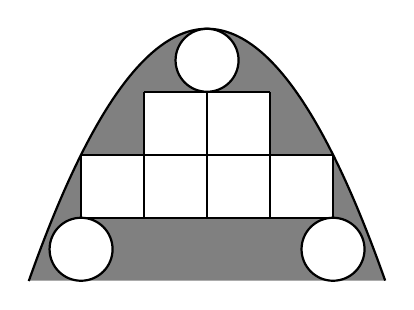
\begin{tikzpicture}[smooth,samples=300,scale=0.8,>=stealth,thick]
			\path
			(-2.83,0) coordinate (A)
			(2.83,0) coordinate (B)
			;
			\fill[gray] (-2.83,0)--plot[domain=-2.83:2.83](\x,{-0.5*(\x)^2+4})--(2.83,0)--cycle;
			\fill[white] (-2,1)--(2,1)--(2,2)--(1,2)--(1,3)--(-1,3)--(-1,2)--(-2,2)--cycle;
			\draw[fill=white] (-2,0.5) circle (0.5) (2,0.5) circle (0.5) (0,3.5) circle (0.5);
			\draw(-2,1) grid (2,2) (-1,2) grid (1,3);
			\draw[domain=-2.83:2.83] plot(\x,{-0.5*(\x)^2+4});
	\end{tikzpicture}}
	\loigiai{
		Gắn hệ trục tọa độ như hình bên, đơn vị trên mỗi trục là 1 m .
		Phương trình Parabol có dạng $y=a x^2+c$.\\
		Do Parabol qua các điểm $(0 ; 4)$ và $(2 ; 2)$ nên ta được $\left\{\begin{array}{l}c=4 \\ 4 a+c=2\end{array} \Rightarrow\left\{\begin{array}{l}a=-\dfrac{1}{2} \\ c=4\end{array}\right.\right.$. Suy ra Parabol: $y=-\dfrac{1}{2} x^2+4$.\\
		Parabol cắt trục hoành tại hai điểm $\mathrm{A}, \mathrm{B}$ có hoành độ là nghiệm của phương trình $-\dfrac{1}{2} x^2+4=0 \Leftrightarrow\left[\begin{array}{l}x=2 \sqrt{2} \\ x=-2 \sqrt{2}\end{array}\right.$. Khi đó hoành độ của A và B lần lượt là $-2 \sqrt{2}$ và $2 \sqrt{2}$.\\
		Diện tích cả cánh cửa là $S=\int\limits_{-2 \sqrt{2}}^{2 \sqrt{2}}\left(-\dfrac{1}{2} x^2+4\right) d x=$.\\
		Diện tích các tấm kính bằng: $6+3 \cdot \pi \cdot\left(\dfrac{1}{2}\right)^2$.\\
		Diện tích phần còn lại là : $\int\limits_{-2 \sqrt{2}}^{2 \sqrt{2}}\left(-\dfrac{1}{2} x^2+4\right) d x-\left[6+3 \cdot \pi \cdot\left(\dfrac{1}{2}\right)^2\right]$.\\
		Giá tiền sơn là $\left\{\int\limits_{-2 \sqrt{2}}^{2 \sqrt{2}}\left(-\dfrac{1}{2} x^2+4\right) d x-\left[6+3 \cdot \pi \cdot\left(\dfrac{1}{2}\right)^2\right]\right\} \cdot 1,2 \approx 8,1$ triệu.
	}
\end{vd}
\dongcham{10}
\begin{vd}%[2D3K3-2]
	\immini{Một chiếc cổng có hình dạng là một Parabol có khoảng cách giữa hai chân cổng là $AB=8$ m. Người ta treo một tấm phông hình chữ nhật có hai đỉnh $M,\,N$ nằm trên Parabol và hai đỉnh $P,\,Q$ nằm trên mặt đất (như hình vẽ). Ở phần phía ngoài phông (phần không tô đen) người ta mua hoa để trang trí với chi phí $1$ m$^2$ cần số tiền mua hoa là $200.000$ đồng, biết $MN=4$ m, $MQ=6$ m. Hỏi số tiền mua hoa trang trí chiếc cổng gần với số tiền nào sau đây?
	}
	{
		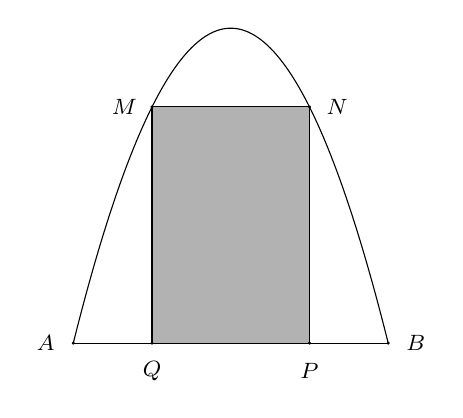
\begin{tikzpicture}[font=\footnotesize, line join=round, line cap=round, >=stealth]
			\begin{scope}[xscale=0.5,yscale=0.5]
				\draw[samples=100,domain=-4:4]plot(\x,{-0.5*(\x)^2+8});
				\path (-2,6)coordinate(M)(2,6)coordinate(N)(-2,0)coordinate(Q)(2,0)coordinate(P)(-4,0)coordinate(A)(4,0)coordinate(B);
				\fill[gray!60,draw=black](M)--(N)--(P)--(Q)--cycle;
				\draw(A)--(B);
				\foreach \d/\g in{A/180,B/0,M/180,N/0,P/-90,Q/-90}
				\draw(\d)circle(0.7pt)node[shift={(\g:0.35)}]{$\d$};
			\end{scope}
		\end{tikzpicture}
	}
	\loigiai{
		\immini{Chọn hệ trục tọa độ như hình vẽ.\\
			Parabol đối xứng qua $Oy$ nên có dạng $(P)\colon y=ax^2+c$.\\
			Vì $(P)$ đi qua $B(4;0)$ và $N(2;6)$ nên $(P)\colon y=-\dfrac{1}{2}x+8$.\\
			Diện tích hình phẳng giới hạn bởi $(P)$ và $Ox$ là
			\[S_1=2\displaystyle\int\limits_{0}^{4} {\left(-\dfrac{1}{2}x^2+8\right)}\mathrm{\,d}x=\dfrac{128}{3}\mathrm{m}^2.\]
			Diện tích phần trồng hoa là \[S=S_1-S_{MNPQ}=\dfrac{128}{3}-24=\dfrac{56}{3}\mathrm{m}^2.\]
			Số tiền dùng để mua hoa là $\dfrac{56}{3}\cdot 200000=3.733.300$ đồng.}
		{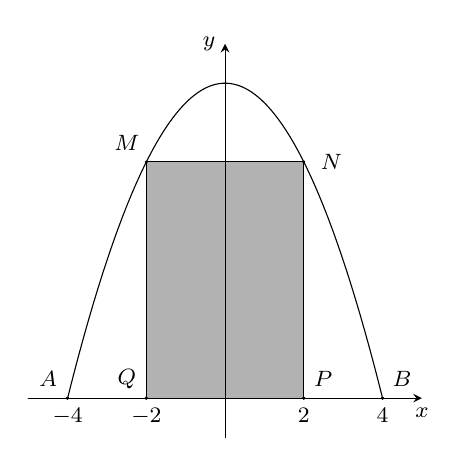
\begin{tikzpicture}[font=\footnotesize, line join=round, line cap=round, >=stealth]
				\begin{scope}[xscale=0.5,yscale=0.5]
					\draw[samples=100,domain=-4:4]plot(\x,{-0.5*(\x)^2+8});
					\path (-2,6)coordinate(M)(2,6)coordinate(N)(-2,0)coordinate(Q)(2,0)coordinate(P)(-4,0)coordinate(A)(4,0)coordinate(B);
					\fill[gray!60,draw=black](M)--(N)--(P)--(Q)--cycle;
					\draw(A)--(B);
					\foreach \d/\g in{A/135,B/45,M/135,N/0,P/45,Q/135}
					\draw(\d)circle(0.7pt)node[shift={(\g:0.35)}]{$\d$};
					\draw [->](-5,0)--(5,0)node[below]{$x$};
					\draw [->](0,-1)--(0,9)node[left]{$y$};
					\foreach \x in{-4,-2,2,4}
					\draw(\x,0)circle(0.7pt)node[below]{$\x$};
				\end{scope}
		\end{tikzpicture}}
	}
\end{vd}\dongcham{15}

\begin{vd} %[Word to LaTeX 3.2]
	\immini{Hình vẽ dưới đây cho biết một miền D (được tô đậm) nằm trong hình vuông cạnh bằng 4, miền D này gồm những điểm có khoảng cách tới tâm hình vuông nhỏ hơn hoặc bằng khoảng cách tới cạnh gần nhất của hình vuông. Tính diện tích miền D, với kết quả làm tròn đến chữ số thập phân thứ nhất.
	}{
		%% cách tường minh hơn
		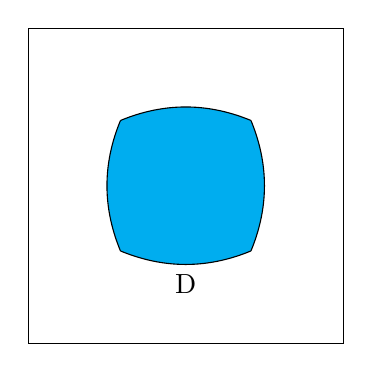
\begin{tikzpicture}
			\pgfmathsetmacro{\can}{-2+2*sqrt(2)}
			\filldraw [cyan] (-\can,-\can) rectangle (\can, \can) ;
			\filldraw [cyan, draw = black, smooth,samples =100, domain=-\can:\can ] plot (\x,{-(0.25)*(\x)^2+1}) ;
			\filldraw [cyan, draw = black,rotate=90, smooth,samples =100, domain=-\can:\can ] plot (\x,{-(0.25)*(\x)^2+1}) ;
			\filldraw [cyan, draw = black,rotate=180, smooth,samples =100, domain=-\can:\can ] plot (\x,{-(0.25)*(\x)^2+1}) ;
			\filldraw [cyan, draw = black,rotate=270, smooth,samples =100, domain=-\can:\can ] plot (\x,{-(0.25)*(\x)^2+1}) ;
			\draw (-2,-2)--(-2,2)--(2,2)--(2,-2)--cycle;
			\node[below] at (0,-1) {D};
		\end{tikzpicture}
	}
	\loigiai{
		\immini{
			Chọn hệ trục tọa độ như hình vẽ. Gọi $M(x,y)$ thuộc đường biên của $D$ (hình vẽ).\\
			Theo giả thiết
			\begin{eqnarray*}
				OM\le MH &\Leftrightarrow&\sqrt{x^2+y^2}\le 2-y\\
				&\Leftrightarrow& x^2+y^2\le 4-4y+y^2 \\
				&\Leftrightarrow& y\le -\dfrac{1}{4}x^2+1
			\end{eqnarray*}
			Suy ra, một phần đường biên của $D$ (phần phía trên) có phương trình $y= -\dfrac{1}{4}x^2+1$.
			
		}{
			\begin{tikzpicture}
				\pgfmathsetmacro{\can}{-2+2*sqrt(2)}
				\filldraw [white] (-\can,-\can) rectangle (\can, \can) ;
				\filldraw [white, draw = black, smooth,samples =100, domain=-\can:\can ] plot (\x,{-(0.25)*(\x)^2+1}) ;
				\filldraw [white, draw = black,rotate=90, smooth,samples =100, domain=-\can:\can ] plot (\x,{-(0.25)*(\x)^2+1}) ;
				\filldraw [white, draw = black,rotate=180, smooth,samples =100, domain=-\can:\can ] plot (\x,{-(0.25)*(\x)^2+1}) ;
				\filldraw [white, draw = black,rotate=270, smooth,samples =100, domain=-\can:\can ] plot (\x,{-(0.25)*(\x)^2+1}) ;
				\fill[pattern=north west lines] (0,1)--plot[domain=0:\can](\x,{-(0.25)*(\x)^2+1})--plot[domain=\can:0](\x,{\x})--cycle;
				\draw (-2,-2)--(-2,2)--(2,2)--(2,-2)--cycle 
				(-2.5,-2.5)--(2.5,2.5)node[below right]{\tiny$y=x$}
				(0,0)--(0.4,0.96)node[above right]{\footnotesize$M$}--(0.4,2)node[above]{\footnotesize$H$};
				\draw[->] (-3,0)--(3,0) node[below]{$x$};
				\draw[->] (0,-2.2)--(0,2.5) node[left]{$y$};
				\draw (0,0) node[below right]{$O$};
		\end{tikzpicture}}
		Phương trình hoành độ giao điểm của đường parabol trên và đường thẳng $y=x$ là:
		$$-\dfrac{1}{4}x^2+1=x\Leftrightarrow x=-2+2\sqrt{2}$$
		Diện tích miền D là: $S=8\left[\displaystyle\int\limits_0^{2\sqrt{2}-2}{\left(-\dfrac{1}{4}x^2+1-x\right)\mathrm{\, d}x}\right]\approx 3,5$.
	}
\end{vd}

\dongcham{11}

\begin{vd}
	\immini{Trong cơ khí chế tạo, một chi tiết máy hình đĩa tròn có dạng như hình vẽ bên, nhận $A B$ và $C D$ làm các trục đối xứng. Người ta cần phủ sơn cả hai mặt của chi tiết. Biết rằng đường tròn lớn có bán kính 5 dm , các đường tròn nhỏ đều có bán kính bằng $2 \mathrm{dm}, A B=C D=4 \mathrm{dm}$ và chi phí sơn là 103.000 đồng $/ \mathrm{m}^2$. Chi phí để sơn hoàn thiện chi tiết máy bằng bao nhiêu nghìn đồng (kết quả được làm tròn đến hàng đơn vị)?
	}{
		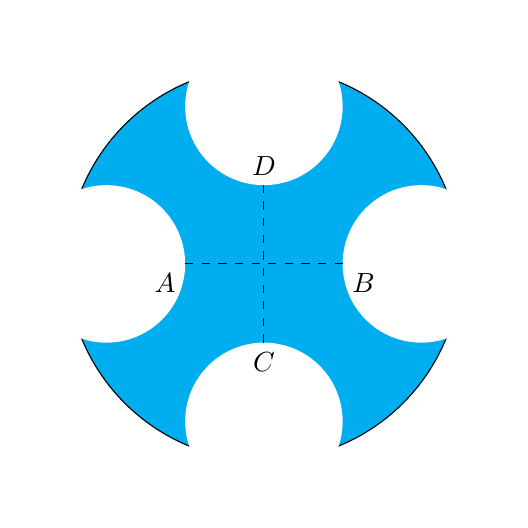
\begin{tikzpicture}[smooth,samples=300,scale=0.5,>=stealth]
			\draw[fill=cyan](0,0) circle (5 cm);
			\fill[white] (4,0) circle (2 cm) (-4,0) circle (2 cm) (0,4) circle (2 cm) (0,-4) circle (2 cm);
			\draw[dashed] (-2,0)node[below left]{$A$}--(2,0)node[below right]{$B$} (0,-2)node[below]{$C$}--(0,2)node[above]{$D$};
	\end{tikzpicture}}
	\loigiai{
		\immini{Gắn hệ trục tọa độ $Oxy$ như hình vẽ. Khi đó:
			\begin{itemize}
				\item [$\bullet$] Phương trình nửa đường tròn lớn phía trên $Ox$ là $y=\sqrt{25-x^2}$
				\item [$\bullet$] Phương trình nửa đường tròn nhỏ phía trên $Ox$ đi qua $B$ là $y=\sqrt{4-(x-4)^2}$
			\end{itemize}
			Phương trình hoành độ giao điểm của chúng
			$$\sqrt{25-x^2}=\sqrt{4-(x-4)^2}\Rightarrow x_0=\dfrac{37}{8}.$$
		}{
			\begin{tikzpicture}[smooth,samples=300,scale=0.5,>=stealth]
				\draw[draw=none,pattern = north west lines] (2,0) plot[domain=2:4.625](\x,{sqrt(-(\x)^2+8*(\x)-12)})--(4.625,0)--cycle;
				\draw[draw=none,pattern = north west lines] (4.625,1.9)--plot[domain=4.625:5](\x,{sqrt(25-(\x)^2)})--(5,0)--(4.625,0);
				\draw[->] (-6,0)--(7.4,0) node[below]{$x$};
				\draw[->] (0,-5.5)--(0,6) node[right]{$y$};
				\draw (0,0) node[above left]{$O$} circle (5 cm);
				\draw[domain=2:4.625] plot(\x,{sqrt(-(\x)^2+8*(\x)-12)});
				\draw[domain=2:4.625,dashed] plot(\x,{-sqrt(-(\x)^2+8*(\x)-12)});
				%\draw[fill=black] (2,-1) circle(1.5pt) (2,0) circle(1pt) (0,-1) circle(1pt);
				\draw[dashed] (4.625,1.9)--(4.625,0)node[below]{\small$x_0$};
				\node[below] at (1.8,0) {$2$};
				\node[below] at (5.4,0) {$5$};
		\end{tikzpicture}}
		Diện tích phần gạch sọc là $S_1=\displaystyle\int\limits_2^{\frac{37}{8}}\sqrt{4-(x-4)^2}\mathrm{\, d}x+\displaystyle\int\limits_{\frac{37}{8}}^5\sqrt{25-x^2}\mathrm{\, d}x$.\\
		Diện tích hình tròn lớn là: $S=\pi\cdot 5^2=25\pi$.
		Diện tích một mặt cần sơn là:
		$$S_2=S-8S_1=25\pi-8\left(\displaystyle\int\limits_2^{\frac{37}{8}}\sqrt{4-(x-4)^2}\mathrm{\, d}x+\displaystyle\int\limits_{\frac{37}{8}}^5\sqrt{25-x^2}\mathrm{\, d}x\right)$$
		Đổi đơn vị: $103000$ đồng/m$^2$=1030 đồng/dm$^2$.\\
		Chi phí sơn hoàn thiện chi tiết máy là: $2\cdot S_2\cdot 1030\approx 82$ (nghìn đồng).
	}
\end{vd}
\dongcham{12}
\boxmini{BÀI TẬP TRẮC NGHIỆM}
\ind{PHẦN I.}{\inden{Câu trắc nghiệm nhiều phương án lựa chọn. Mỗi câu hỏi thí sinh chỉ chọn một phương án.}} 
\setcounter{ex}{0}
\Opensolutionfile{ans}[ans/2D4-B3-d1-1]
\begin{ex}
	Tính diện tích hình phẳng giới hạn bởi đồ thị hàm số $y=x^3$, trục hoành và hai đường thẳng $x=1$, $x=3$.
	\choice
	{$19 $}
	{$18 $}
	{$\dfrac{2186}{7}\pi $}
	{\True $20 $}
	\loigiai{
		$S=\displaystyle \int\limits_1^3 |x^3|\mathrm{\,d}x=\left|\displaystyle \int\limits_1^3 x^3 \mathrm{\,d} x\right|=20.$
	}
\end{ex}\cham{3}

\begin{ex}
	Diện tích hình phẳng giới hạn bởi đồ thị các hàm số $y=\sin x;y=0;x=0$ và $x=2\pi$ là
	\choice
	{\True $4$}
	{$1$}
	{$2$}
	{$0$}
	\loigiai{
		\immini{Diện tích hình phẳng được tính bởi\\ $I=2\displaystyle\int\limits_{0}^{\pi}(\sin x-0)\mathrm{\,d}x= 2\left.(-\cos x)\right|_0^\pi =4$.\\
		}
		{
			\begin{tikzpicture}
				\draw[->,line width = 1pt] (-0.5,0)--(0,0) node[below right]{$O$}--(7,0) node[below]{$x$};
				\draw[->,line width = 1pt] (0,-1.2) --(0,2) node[right]{$y$};
				\draw[smooth,samples=100,domain=-0.5:6.6] plot(\x,{sin(\x r)});
				\draw[draw=none,pattern = north west lines] (0,0) plot[domain=0:6.28](\x,{sin(\x r)}) (6.28,0)--(0,0);
				\draw (3.14,0) node[below]{$\pi$} circle (1pt);
				\draw (6.28,0) node[below]{} circle (1pt);
				\draw (6.4,0) node[below]{$2\pi$};
			\end{tikzpicture}
		}
	}
\end{ex}\cham{4}

\begin{ex}%[2D3Y3-1]%
	Gọi $S$ là diện tích hình phẳng giới hạn bởi các đường $y=3^x$, $y=0$, $x=0$, $x=2$. Mệnh đề nào dưới đây đúng?
	\choice
	{\True $S=\displaystyle \int_0^2 3^x\mathrm{\,d}x$}
	{$S=\pi \displaystyle \int_0^2 3^{2x}\mathrm{\,d}x$}
	{$S=\displaystyle \int_0^2 3^{2x}\mathrm{\,d}x$}
	{$S=\pi \displaystyle \int_0^2 3^x\mathrm{\,d}x$}
	\loigiai{
		Ta có $S=\displaystyle \int_0^2 \left|3^x\right|\mathrm{\,d}x=\displaystyle \int_0^2 3^x\mathrm{\,d}x$.
	}
\end{ex}\cham{4}

\begin{ex}%[Ngọc Hiếu, dự án Thi HK2_Latex1920]%[2D3B3-1]%
	Tính diện tích $S$ của hình phẳng giới hạn bởi đồ thị các hàm số $y=3x^2$, $y=2x+5$, $x=-1$ và $x=2$.
	\choice
	{$S=27$}
	{$S=\dfrac{256}{27}$}
	{\True $S=\dfrac{269}{27}$}
	{$S=9$}
	\loigiai{
		Xét phương trình hoành độ giao điểm của hai đồ thị $3x^2=2x+5\Leftrightarrow 3x^2-2x-5=0$. Phương trình có hai nghiệm $x=-1$, $x=\dfrac{5}{3}$.\\
		Diện tích của hình phẳng cần tìm là $S=\displaystyle \int\limits_{-1}^{2} |(3x^2-2x-5)| \mathrm{d}x$ $=\Big|\displaystyle \int\limits_{-1}^{\frac{5}{3}} (3x^2-2x-5) \mathrm{d}x \Big|$ $+\Big|\displaystyle \int\limits_{\frac{5}{3}}^{2} (3x^2-2x-5) \mathrm{d}x \Big|$ $=\Big| \left(x^3-x^2-5x\right) \Big|_{-1}^{\frac{5}{3}} \Big|$ $+\Big| \left(x^3-x^2-5x\right) \Big|_{\frac{5}{3}}^2 \Big|$ $=\Big| -\dfrac{175}{27} - 3 \Big| +\Big|-6 + \dfrac{175}{27} \Big|=\dfrac{269}{27}$.
	}
\end{ex}\cham{4}

\begin{ex}%[2D3B3-1]%
	Tính diện tích $(S)$ của hình phẳng giới hạn bởi các đồ thị hàm số $y=x^2-x$, $y=2x+4$ và các đường thẳng thẳng $x=1$, $x=4$.
	\choice
	{$S=\dfrac{1539}{10}$}
	{\True $S=\dfrac{27}{2}$}
	{$S=\dfrac{125}{6}$}
	{$S=\dfrac{81}{2}$}
	\loigiai
	{
		Phương trình hoành độ giao điểm của hai đồ thị hàm số là
		\begin{eqnarray*}
			x^2-x=2x+4 \Leftrightarrow x^2-3x-4=0 \Leftrightarrow \left[\begin{aligned}&x=-1 \\&x=4.\end{aligned}\right.
		\end{eqnarray*}
		Diện tích hình phẳng cần tìm là
		\[S=\displaystyle\int\limits_1^4\left|\left(x^2-x\right)-(2x+4)\right|\mathrm{\,d}x = \displaystyle\int\limits_1^4\left|x^2-3x-4\right|\mathrm{\,d}x = \left|\displaystyle\int\limits_1^4\left(x^2-3x-4\right)\mathrm{\,d}x\right| = \dfrac{27}{2}.\]
	}
\end{ex}\cham{4}


\begin{ex}%[Lê Đăng Phong, dự án Thi HK2_Latex1920]%[2D3B3-1]%
	Tính diện tích $S$ của hình phẳng giới hạn bởi các đường $y=x^2-x$, $y=x+3$.
	\choice
	{\True $ \dfrac{32}{3}$}
	{$ \dfrac{16}{3}$}
	{$ \dfrac{16}{3}$}
	{$ \dfrac{2}{3}$}
	\loigiai{
		$x^2-x=x+3 \Leftrightarrow x^2-2x-3=0\Leftrightarrow \hoac{&x=-1\\&x=3.}$\\
		Diện tích $S$ là
		$$S=\displaystyle\int\limits_{-1} ^3  \left| x^2-2x-3\right| \textrm{\,d}x = -\displaystyle\int\limits_{-1} ^3 \left(  x^2-2x-3\right)  \textrm{\,d}x  = \dfrac{32}{3}.$$
	}
\end{ex}\cham{6}

%Từ ngân hàng. Câu 157451. File gốc: H:\My Drive\NGUON-CODE2021\Question Bank\[2D3B3-1].tex
\begin{ex}%[Đề KSCL 2017 - 2018 Sở giáo dục và đào tạo Yên Bái]%[Minh Ha Trieu, dự án(12EX-10)]%[2D3B3-1]%
	Tính diện tích hình phẳng giới hạn bởi đồ thị các hàm số $y=-x^2+2x$ và $y=-3x$.
	\choice
	{$\dfrac{125}{2}$}
	{$\dfrac{125}{3}$}
	{\True $\dfrac{125}{6}$}
	{$\dfrac{125}{8}$}
	\loigiai
	{Phương trình hoành độ giao điểm $-x^2+2x=-3x\Leftrightarrow\hoac{&x=0\\&x=5.}$\\
		Khi đó diện tích $S$ của hình phẳng được xác định bởi
		$$S=\displaystyle\int \limits_0^5|-x^2+2x+3x|\mathrm{\, d}x=\displaystyle\int\limits_0^5|-x^2+5x|\mathrm{\, d}x=\left| \displaystyle\int\limits_0^5(-x^2+5x)\mathrm{\, d}x\right|
		=\left| \left(-\dfrac{x^3}{3}+\dfrac{5x^2}{2}\right)\Big| _0^5\right| =\dfrac{125}{6}.$$
	}
\end{ex}\cham{6}

\begin{ex}%[KSCL giữa HK2 Cụm trường THPT TP Nam Định]%[Nguyễn Tiến, 12EX7]%[2D3B3-1]%
	\immini[thm]{
		Đồ thị trong hình bên dưới là của hàm số $ y=f(x)$. Gọi $S$ là diện tích hình phẳng (phần gạch chéo trong hình), chọn khẳng định đúng.
		\choice
		{$S=\displaystyle\int\limits_{-2}^0 f(x)\mathrm{\,d}x +\int\limits_0^1 f(x)\mathrm{\,d}x$}
		{\True $S=\displaystyle\int\limits_{-2}^0 f(x)\mathrm{\,d}x -\int\limits_0^1 f(x)\mathrm{\,d}x$}
		{$S=\displaystyle\int\limits_0^{-2} f(x)\mathrm{\,d}x +\int\limits_0^1 f(x) \mathrm{\,d}x$}
		{$S=\displaystyle\int\limits_{-2}^1 f(x)\mathrm{\,d}x$}}{
		\begin{tikzpicture}[scale=0.7, font=\footnotesize, line join=round, line cap=round, >=stealth]
			\def\a{1} \def\b{1} \def\c{-2}
			\def\xt{-3} \def\xp{2} \def\yt{3} \def\yd{-2}
			\draw[->] (\xt,0)--(\xp,0) node [below]{$x$};
			\draw[->] (0,\yd)--(0,\yt) node [left]{$y$};
			\node at (0,0) [below left]{$O$};
			\node at (1,0) [below right]{$1$};
			\node at (-2,0) [above left]{$-2$};
			\clip (\xt-0.1,\yd+0.1) rectangle (\xp-0.1,\yt-0.1);
			\draw[smooth,samples=300] plot(\x,{\a*(\x)^3+\b*(\x)^2+\c*(\x)});
			\draw[pattern = north east lines, line width = 1.2pt,draw=none](1,0)-- plot[domain=1:-2] (\x,{\a*(\x)^3+\b*(\x)^2+\c*(\x)}) --(-2,0);
	\end{tikzpicture}}
	\loigiai{
		Từ đồ thị ta có $ f(x)\ge 0,\forall x\in [-2;0]$ và $ f(x)\le 0,\forall x\in [0;1]$.\\
		Do đó $S=\displaystyle\int\limits_{-2}^1 \left|f(x)\right|\mathrm{\,d}x=\int\limits_{-2}^0 \left|f(x)\right| \mathrm{\,d}x + \int\limits_0^1 \left|f(x)\right|\mathrm{\,d}x=\int\limits_{-2}^0 f(x)\mathrm{\,d}x -\int\limits_0^1 f(x)\mathrm{\,d}x$.
	}
\end{ex}\cham{2}

\begin{ex}%[2D3B3-1]
	\immini[thm]
	{
		Diện tích hình phẳng gạch sọc trong hình vẽ bên bằng
		\choice
		{$ \displaystyle\int\limits_{3}^{1} 2^x \mathrm{\,d}x $}
		{$ \displaystyle\int\limits_{1}^{3} 2^x \mathrm{\,d}x $}
		{$ \displaystyle\int\limits_{3}^{1} (2^x-2) \mathrm{\,d}x $}
		{\True $ \displaystyle\int\limits_{1}^{3} (2^x-2) \mathrm{\,d}x $}
	}
	{
		\begin{tikzpicture}[scale=0.55, font=\footnotesize, line join=round, line cap=round,x=1cm,y=0.5cm,>=stealth]
			\draw[->] (-1,0) -- (4,0) node[below] {\scriptsize $x$};
			\draw[->] (0,-1) -- (0,9.2) node[left] {\scriptsize $y$};
			\draw (0,0)node[below left]{\scriptsize $O$};
			\draw (1,0)circle(1.25pt)node[below]{\scriptsize $1$}--(1,2)--(0,2)circle(1.25pt)node[left]{\scriptsize $2$}--(3,2);
			\draw (3,0)circle(1.25pt)node[below]{\scriptsize $3$}--(3,8)--(0,8)circle(1.25pt)node[left]{\scriptsize $8$};
			\draw (3,8.1)node[above]{\scriptsize $ y=2^x $};
			\draw[samples=150,smooth,domain=-1:3.1] plot(\x,{2^(\x)});
			\fill[pattern=north east lines] (1,2)--plot[domain=1:3](\x,{2^(\x)})--(3,2)--cycle;
		\end{tikzpicture}
		
	}
	\loigiai{
		Diện tích phần gạch sọc trong hình vẽ trên là diện tích hình phẳng được giới hạn bởi các đường $ y=2^x $, $ y=2 $, $ x=1 $ và $ x=3 $. Do vậy, diện tích cần tìm bằng $ \displaystyle\int\limits_{1}^{3} (2^x-2) \mathrm{\,d}x $.
		
	}
\end{ex}\cham{2}

\begin{ex}%[Dự án tool4Latex-Lần 1 - Phat Dang Tan - Đề 25]%[2D3B3-1]
	\immini[thm]{Diện tích phần hình phẳng gạch chéo trong hình vẽ bên được tính theo công thức nào dưới đây?
		\choice
		{$\displaystyle\int\limits_{-1}^2\left(2x^2-2x-4\right)\mathrm{\,d}x$ }
		{$\displaystyle\int\limits_{-1}^2\left(-2x+2\right)\mathrm{\,d}x$ }
		{$\displaystyle\int\limits_{-1}^2\left(2x-2\right)\mathrm{\,d}x$ }
		{\True $\displaystyle\int\limits_{-1}^2\left(-2x^2+2x+4\right)\mathrm{\,d}x$}}{
		\begin{tikzpicture}[>=stealth,line join=round,line cap=round,font=\footnotesize,scale=0.6]
			\def\f(#1){-(#1)^2 + 3}
			\def\g(#1){(#1)^2 - 2*(#1) -1}
			\fill[pattern=north west lines, opacity=0.5] plot[smooth,samples=200,domain=-1:2] (\x,{\f(\x)})--plot[smooth,samples=200,domain=2:-1] (\x,{\g(\x)})--cycle;
			
			\draw[color=black,thick, smooth, samples=200, domain= -1.3:2.4] plot(\x,{\f(\x)}) node[below right]{$y=-x^2 +3$};
			\draw[color=black,thick, smooth, samples=200, domain= -1.2:2.54] plot(\x,{\g(\x)}) node[above right]{$y=x^2 -2x-1$};
			
			\draw[->] (-1.5,0)--(5,0) node[below]{$x$};
			\draw[->] (0,-2.5)--(0,3.5) node[left]{$y$};
			\fill[name=O] (0,0) circle (1pt) node[below right] {$O$}; 
			
			\coordinate[label=below:{$-1$}] (-1x) at (-1,0);
			\coordinate[label=above:{$2$}] (2x) at (2,0);
			
			\draw[dashed] (-1,0)--(-1,{\f(-1)}) (2,0)--(2,{\f(2)});
			\foreach \p in {-1x,2x}
			\fill (\p) circle (1.1pt);
	\end{tikzpicture}}
	\loigiai{
		$S=\displaystyle\int\limits_{-1}^2 \left|\left(-x^2+3\right) - \left(x^2 -2x -1\right)\right|\mathrm{\,d}x=\displaystyle\int\limits_{-1}^2 \left(-x^2 +3 -x^2 +2x +1\right)\mathrm{\,d}x=\displaystyle\int\limits_{-1}^2 \left(-2x^2 + 2x +4\right)\mathrm{\,d}x$.
	}
\end{ex}\cham{2}

\begin{ex}%[Đề thi giữa kì 2 THPT Việt Đức, Hà Nội (2019)]%[2D3B3-1]%
	\immini[thm]{
		Cho $(\mathcal{H})$ là hình phẳng giới hạn bởi $y=\sqrt{x}, y=x-2$ và trục hoành (hình vẽ). Diện tích của $(\mathcal{H})$ bằng
		\haicot
		{$\dfrac{16}{3}$}
		{\True $\dfrac{10}{3}$}
		{$\dfrac{7}{3}$}
		{$\dfrac{8}{3}$}
	}{
		\begin{tikzpicture}[scale=0.8, font=\footnotesize, line join=round, line cap=round, >=stealth]
			\draw[->,line width = 1pt] (-0.5,0) node[below]{$O$}--(5,0) node[below]{$x$};
			\draw[->,line width = 1pt] (0,-1.5) --(0,3) node[right]{$y$};
			\draw (2,0) node[below]{$2$} circle (1pt);
			\draw [samples=100, domain=0:4.5] plot (\x, {(\x)^0.5}) node at (2.8,1.8)[left]{$f(x)=\sqrt{x}$};
			\draw [samples=100, domain=0.5:4.5] plot (\x, {(\x)-2}) node at (1,-1) [right]{$g(x)=x-2$};
			\draw[pattern = north east lines, line width = 1.2pt,draw=none] (-1,-2)
			plot[domain=0:4] (\x, {(\x)^0.5}) -- (4,2)--(2,0)--cycle;
			\draw[dashed](4,0)node[below]{$4$}circle (1pt)--(4,2);
		\end{tikzpicture}
	}
	\loigiai
	{
		Phương trình hoành độ giao điểm của $f(x)$ và $g(x)$ là $\sqrt{x}=x-2\Leftrightarrow\heva{& x-2\geq 0\\ & x=(x-2)^2}\Leftrightarrow x=4$.\\
		Do đó diện tích $S$ của $(\mathcal{H})$ là $S=\displaystyle\int\limits_{0}^{2} \sqrt{x} \mathrm{\,d}x+\displaystyle\int\limits_{2}^{4} (\sqrt{x}-x+2) \mathrm{\,d}x=\dfrac{10}{3}$.
	}
\end{ex}\cham{2}

\begin{ex}%[2D3K3-1]
	\immini[thm]{
		Cho parabol $(P)$ có đồ thị như hình vẽ. Tính diện tích hình phẳng giới hạn bởi $(P)$ và trục hoành.
		\choice
		{$1$}
		{$2$}
		{$\dfrac{5}{3}$}
		{\True $\dfrac{4}{3}$}
	}{
		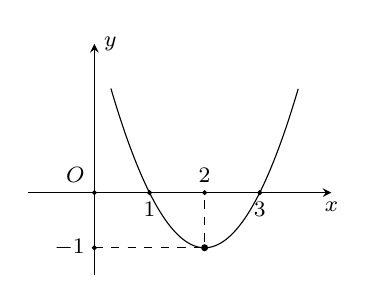
\begin{tikzpicture}[>=stealth, scale=0.7,font=\footnotesize]
			\draw[->](-1.2,0)--(4.3,0) node[below]{$x$};
			\draw[->] (0,-1.5)--(0,2.7) node[right]{$y$};
			\draw[smooth, samples=200, domain=0.3:3.7] plot(\x,{(\x)^2-4*(\x)+3});
			\draw (1,0) node[below]{$1$} (0,0) node[above left]{$O$} (0,-1) node[left]{$-1$} (2,0) node[above]{$2$} (3,0) node[below]{$3$};
			\draw[dashed] (0,-1)--(2,-1)--(2,0);
			\draw[fill=black] (0,0) circle(1pt) (1,0) circle (1pt) (2,0) circle (1pt) (2,-1) circle (1.5pt) (3,0) circle (1pt) (0,-1) circle (1pt);
		\end{tikzpicture}
	}
	\loigiai{
		Parabol đã cho có dạng $y=f(x)=ax^2+bx+c$, $a\ne 0$. Vì $(P)$ cắt trục hoành tại các điểm $(1;0)$, $(3;0)$ và đi qua điểm $(2;-1)$ nên ta có
		\begin{align*}
			\heva{&f(1)=f(3)=0\\ &f(2)=-1}\Leftrightarrow \heva{&a=1\\ &b=-4\\ &c=3.}
		\end{align*}
		Dựa vào đồ thị của $(P)$, ta có diện tích hình phẳng cần tìm là
		\begin{align*}
			-\displaystyle\int\limits_{1}^{3}\left( x^2-4x+3 \right)\mathrm{\,d}x= -\left( \dfrac{x^3}{3}-2x^2+3x \right)\Bigg|_1^3=\dfrac{4}{3}.
		\end{align*}
	}
\end{ex}\cham{2} 

\begin{ex}
	\immini[thm]{
		Cho hình vuông $OABC$ có cạnh bằng $4$ được chia thành hai phần bởi đường cong $(C)$ có phương trình $y=0{,}25x^{2}$. Gọi $S_{1}$, $S_{2}$ lần luợt là diện tích của phần không bị gạch và phần bị gạch (như hình vẽ bên). Tỉ số $\dfrac{S_{1}}{S_{2}}$ bằng
		\choice
		{$1$}
		{\True $2$}
		{$1{,}5$}
		{$\dfrac{1}{2}$}
	}{
		\begin{tikzpicture}[scale=0.9, line join=round, line cap=round,>=stealth]
			\draw [->] (-0.5,0) -- (4.5,0) node[below]{$x$};
			\draw [->] (0,-0.5) -- (0,4.5) node[left]{$y$};
			\draw (0,0) node[below left]{$O$} circle(1pt);
			\draw[dashed] (4,0)|-(0,4)node[above right]{$A$}(4,4)node[right]{$B$}(4,4.3)node[above]{$(C)$}(2,2)node[above]{$S_1$}(3,1)node[above]{$S_2$};
			\draw [smooth,domain=0:4.2, samples=300, thick] plot(\x,{0.25*(\x)^2});
			\fill(0,4)circle(1pt) node[left]{$4$}(4,0)circle(1pt) node[below]{$4$}node[above right]{$C$};
			\fill [pattern = north east lines] plot[domain=0:4] (\x,{0.25*(\x)^2})--(4,4)--(4,0)--cycle;
		\end{tikzpicture}
	}
	\loigiai{
		$$S_2=\displaystyle\int\limits_{0}^{4}0{,}25x^2\,\mathrm{d}x
		=\dfrac{16}{3}.$$
		$$S_1=S_{OABC}-S_2=16-\dfrac{16}{3}=\dfrac{32}{3}.$$
		$\Rightarrow\dfrac{S_1}{S_2}=2$.
	}
\end{ex}\cham{3}

\begin{ex}%[2D3T3-2]
	\immini[thm]{Ông A muốn làm cửa sắt được thiết kế như hình bên. Vòm cổng có hình dạng một parabol. Giá $1$m$^2$ cửa sắt là $660000$ đồng. Cửa sắt có giá (nghìn đồng) là
		\choice
		{$6500$}
		{$\dfrac{55}{6}\cdot 10^3$}
		{$5600$}
		{\True $6050$}}
	{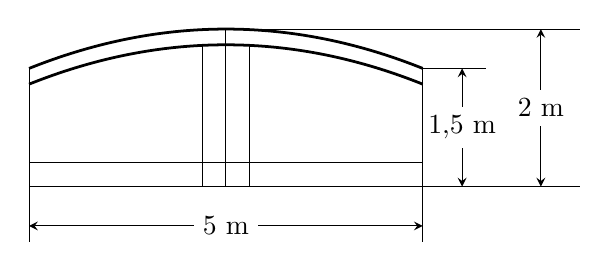
\begin{tikzpicture}[>=stealth, scale=1]
			\draw[line width=1pt,smooth,samples=100,domain=-2.5:2.5] plot(\x,{-0.08*(\x)^2+2});
			\draw[line width=1pt,smooth,samples=100,domain=-2.5:2.5] plot(\x,{-0.08*(\x)^2+1.8});
			\draw[<->] (3,0)--(3,1.5) node[midway, fill=white] {$1{,}5$ m};
			\draw[<->] (4,0)--(4,2) node[midway, fill=white] {$2$ m};
			\draw[<->] (-2.5,-.5)--(2.5,-.5) node[midway, fill=white] {$5$ m};
			\draw (-2.5,1.5) -- (-2.5,-0.7) (2.5,1.5) -- (2.5,-0.7) (-2.5,0) -- (4.5,0) (0,2) -- (0,0) (0.3,1.8) -- (0.3,0) (-0.3,1.8) -- (-0.3,0) (-2.5,.3) -- (2.5,0.3) (0,2)--(4.5,2) (2.5,1.5)--(3.3,1.5);
	\end{tikzpicture}}
	\loigiai{
		\immini{Chọn hệ trục tọa độ $Oxy$ như hình vẽ. Khi đó, vòm cửa là một parabol có phương trình dạng $y=ax^2+2$.\\
			Vì parabol đi qua điểm $(2,5;1.5)$ nên ta có $1{,}5=a\cdot \left(\dfrac{5}{2}\right)^2+2 \Leftrightarrow a=-\dfrac{2}{25}$.\\
			Như vậy $y=-\dfrac{2}{25}x^2+2$.
		}
		{\begin{tikzpicture}[>=stealth, scale=1]
				\draw[line width=1pt,smooth,samples=100,domain=-2.5:2.5] plot(\x,{-0.08*(\x)^2+2});
				\draw (-2.5,1.5) -- (-2.5,0) (2.5,1.5) -- (2.5,0);
				\draw[->](-3,0)--(3,0) node[below] {$x$};
				\draw[->](0,-1)--(0,3) node[left] {$y$};
				\draw (0.2,-.2) node {$O$};
				\draw (-2.5,0)node[below]{\footnotesize $-\dfrac{5}{2}$} (2.5,0)node[below]{\footnotesize $\dfrac{5}{2}$}; 
				\draw (0,1.5) node[below left] {\footnotesize $1{,}5$};
				\draw (0,2) node[above left] {\footnotesize$2$};
				\draw[dashed] (2.5,1.5)--(-2.5,1.5);
				\fill (0,0) circle(1pt);
				\fill (-2.5,0) circle(1pt);
				\fill (2.5,0) circle(1pt);
				\fill (0,1.5) circle(1pt);
				\fill  (0,2) circle(1pt);
		\end{tikzpicture}}
		\noindent
		Diện tích của cửa sắt là
		$$S=\displaystyle\int\limits_{-\frac{5}{2}}^{\frac{5}{2}}\left(-\dfrac{2}{25}x^2+2\right)\mathrm{\,d}x=\dfrac{55}{6}\;\left(\text{m}^2\right).$$
		Vậy, giá tiền cửa sắt là
		$$\dfrac{55}{6}\cdot 660000=6050000 \;\left(\text{đồng}\right)=6050 \;\left(\text{nghìn đồng}\right). $$	
	}
\end{ex}\cham{6}

\begin{ex}%[Thi thử,Quảng Xương 1-Thanh Hóa-L3, 2019]%[Lê Quốc Hiệp, 12EX8-2019]%[2D3K3-2]%
	\immini[thm]
	{Một viên gạch hoa hình vuông cạnh $80$ cm. Người thiết kế đã sử dụng bốn đường parabol có chung đỉnh tại tâm của viên gạch để tạo ra bốn cánh hoa (phần gạch sọc như hình vẽ bên). Diện tích mỗi cánh hoa của viên gạch bằng
		\choice
		{$\dfrac{800}{3}$ cm$^2$}
		{$\dfrac{400}{3}$ cm$^2$}
		{$250$ cm$^2$}
		{\True $\dfrac{1600}{3}$ cm$^2$}
	}
	{\begin{tikzpicture}[line cap=round,line join=round,font=\footnotesize,>=stealth,scale=1]
			\def\r{2*sqrt(2))}
			\fill (0,0) coordinate (O) circle(1pt)
			(-45:{\r}) coordinate (A) circle(1pt)
			(45:{\r}) coordinate (B) circle(1pt)
			(135:{\r}) coordinate (C) circle(1pt)
			(225:{\r}) coordinate (D) circle(1pt);
			\foreach \x in {B,C,D,A}{
				\draw [name path=n] (O) parabola (\x);
				\draw [name path=m,rotate=45,xscale=-1,rotate=-45] (O) parabola (\x);
				\tikzfillbetween[of=m and n] {pattern=north west lines};
			}
			\draw (A)|-(C)|-(A);
	\end{tikzpicture}}
	\loigiai
	{
		\immini
		{Chọn hệ trục tọa độ như hình vẽ bên, với $A(40;40)$.\\
			Parabol đi qua gốc tọa độ $O$ và điểm $A$ có phương trình dạng $(P)\colon y=ax^2$.\\
			$(P)$ qua $A(40;40)\Rightarrow 40=a\cdot40^2\Rightarrow a=\dfrac{1}{40}$.\\
			Đường thẳng $OA$ có phương trình $y=x$.\\
			Diện tích phần cánh hoa ở góc phần tư thứ nhất là
			\[S_1=2\displaystyle\int\limits_0^{40}\left(x-\dfrac{x^2}{40}\right)\mathrm{\,d}x=2\cdot\left(\dfrac{x^2}{2}-\dfrac{x^3}{120}\right)\bigg|_0^{40}=\dfrac{1600}{3}\text{ cm}^2.\]
		}
		{\begin{tikzpicture}[line cap=round,line join=round,font=\footnotesize,>=stealth,scale=1]
				\draw[->] (-3,0)--(3,0) node[above] {$x$};
				\draw[->] (0,-3)--(0,3) node[left] {$y$};
				\def\r{2*sqrt(2))}
				\fill (0,0) coordinate (O) circle(1pt)
				(-45:{\r}) coordinate (A)  circle(1pt)
				(45:{\r}) coordinate (B) node [right] {$A$} circle(1pt)
				(135:{\r}) coordinate (C) circle(1pt)
				(225:{\r}) coordinate (D) circle(1pt);
				\foreach \x in {B,C,D,A}{
					\draw [name path=n] (O) parabola (\x);
					\draw [name path=m,rotate=45,xscale=-1,rotate=-45] (O) parabola (\x);
					\tikzfillbetween[of=m and n] {pattern=north west lines};
				}
				\draw (-0.2,-0.2) node [below left,fill=white,scale=0.75] {$O$};
				\draw (A)|-(C)|-(A) (0,0)--(B);
		\end{tikzpicture}}
	}
\end{ex}
\cham{4}
\begin{ex}%[Ân Trương - DA1]%[2D3K3-2]%
	\immini[thm]
	{
		Một viên gạch hình vuông cạnh bằng $ 10 \mathrm{~cm} $. Người ta tạo kiểu dáng bằng cách vẽ hình dạng parabol và tô màu phần còn lại như hình vẽ. Biết $ AB=5 \mathrm{~cm},OH=4 \mathrm{~cm} $, giá thành phẩm của phần tô màu là $ 200 $ đồng $ / \mathrm{cm}^{2} $ và phần không tô là $ 100 $ đồng $ / \mathrm{cm}^{2} $. Giá thành phẩm của viên gạch (làm tròn) gần bằng với giá trị nào sau đây?
		\choice
		{\True$14700$ đồng}
		{$16000$ đồng}
		{$16500$ đồng}
		{$15500$ đồng}
	}
	{
		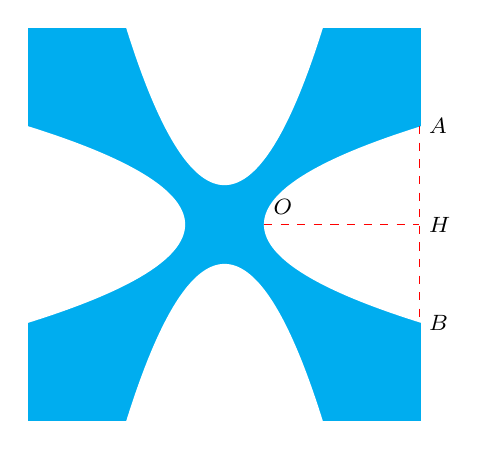
\begin{tikzpicture}[>=stealth,x=1cm,y=1cm,scale=0.5,font=\footnotesize]
			\def\hsf(#1){(#1)*(#1)*16/25}
			%Vẽ Parabol, đường thẳng:
			\draw[fill=cyan, draw=none] (-5,-5) rectangle (5,5);
			\begin{scope}
				\clip (-5,-5) rectangle (5,5);
				\draw [fill=white, draw=none,domain=-3:3, samples=100] plot (\x, {\hsf(\x)+1});
				\draw [fill=white, draw=none,domain=-3:3, samples=100] plot ({\hsf(\x)+1}, \x);
				\draw [fill=white, draw=none,domain=-3:3, samples=100] plot (\x, {-\hsf(\x)-1});
				\draw [fill=white, draw=none,domain=-3:3, samples=100] plot ({-\hsf(\x)-1}, \x);
			\end{scope}
			\path
			(4.95,0) coordinate (H)node[right]{$ H $}
			(1,0) coordinate (O)node[above right]{$ O$}
			(4.95,2.5) coordinate (A)node[right]{$ A$}
			(4.95,-2.5) coordinate (B)node[right]{$ B $};
			\draw[red,dashed](A)--(B)(O)--(H);
		\end{tikzpicture}
	}
	\loigiai{
		Chọn hệ tọa độ $ Oxy $ sao cho tia $ Oy$ trùng với tia $ OH $.\\
		Trong mặt phẳng $ Oxy $, ta thấy phương trình của Parabol có đỉnh $ O $ và đi qua hai điểm $ A\left(-\dfrac{5}{2} ; 4\right) ; B\left(\dfrac{5}{2} ; 4\right) $ là $ y=\dfrac{16}{25} x^{2} $. Gọi $ S_1,S_2 $ lần lượt là diện tích của phần không tô màu và diện tích của phần tô màu, ta có:\\
		$ \heva{& S_{1}=4 \displaystyle\int\limits_{-\frac{5}{2}}^{\frac{5}{2}}\left(4-\dfrac{16}{25} x^{2}\right)  \mathrm{d} x=\dfrac{160}{3}\left(\mathrm{~cm}^{2}\right) \\ & S_{2}=10^{2}-S_{1}=\dfrac{140}{3}\left(\mathrm{~cm}^{2}\right).} $\\
		Vậy, giá viên gạch là: $ T=100 S_{1}+200 S_{2} \approx 14667 $.}
\end{ex}
\cham{7}
\begin{ex}%[THPT Kim Liên]%[Nguyễn Thế Út, dự án W-T-Begin-lần 3]%[2D3K3-2]%
	\immini[thm]
	{
		Một hoa văn trang trí được tạo ra từ một miếng bìa mỏng hình vuông cạnh $20$ cm bằng cách khoét đi bốn phần bằng nhau có hình dạng một nửa elip như hình bên. Biết một nửa trục lớn $AB=6$ cm, trục bé $CD=8$ cm. Diện tích bề mặt hoa văn đó bằng
		\choice
		{\True $400-48\pi (cm^2)$}
		{$400-24\pi (cm^2)$}
		{$400-36\pi (cm^2)$}
		{$400-96\pi (cm^2)$}
	}
	{
		\begin{tikzpicture}[scale=1, font=\footnotesize, line join=round, line cap=round, >=stealth]
			\tkzInit[xmin=-1,xmax=6,ymin=-1,ymax=6]
			%\tkzGrid
			%\tkzAxeXY
			\tkzDefPoints{0/0/I, 5/0/J, 3.5/2.5/A, 5/2.5/B, 5/3.5/C, 5/1.5/D}
			\tkzDrawSquare(I,J)
			\draw (5,1.5) arc (-90:-270:1.5 cm and 1 cm);%ok
			\draw (0,3.5) arc (90:-90:1.5 cm and 1 cm);%ok
			\draw (3.5,0) arc (0:180:1 cm and 1.5 cm);%ok
			\draw (3.5,5) arc (0:-180:1 cm and 1.5 cm);
			\draw[dashed] (0,2.5) -- (5,2.5);
			\draw[dashed] (2.5,0) -- (2.5,5);
			\tkzDrawPoints[fill=black](A,B,C,D)
			\tkzLabelPoints[above left](A,B,C,D)
		\end{tikzpicture}
	}
	\loigiai{
		\textbf{Cách $1$.}
		\immini
		{
			Chọn hệ trục $Oxy$ như hình vẽ ta có $(E)$ qua 3 điểm $A,C,D$ có bán trục lớn $a=6$ và bán trục bé $b=4$, phương trình $(E) \colon \dfrac{x^2}{36}+\dfrac{y^2}{16}=1$.\\
			Diện tích phần hình $ACD$ bằng hai lần diện tích phần $ABC$ có $y>0 \Rightarrow y=4\sqrt{1-\dfrac{x^2}{36}}$. \\
			Vậy diện tích phần $ABC$ là $$S=\displaystyle\int\limits_{-6}^0 4\sqrt{1-\dfrac{x^2}{36}}\mathrm{\,d}x .$$
			Đặt $x=6\sin t \Rightarrow \mathrm{\,d}x=6\cos t\mathrm{\,d}t$ \\
			Đổi cận $ \hoac{&x=-6\Rightarrow t=-\dfrac{\pi}{2}\\&x=0\Rightarrow t=0.} $
		}
		{
			\begin{tikzpicture}[scale=1, font=\footnotesize, line join=round, line cap=round, >=stealth]
				\tkzInit[xmin=-1,xmax=7.5,ymin=-1,ymax=6.5]
				\draw[->,line width = 1pt] (2.5,2.5)--(7,2.5) node[below]{$x$};
				\draw[->,line width = 1pt] (5,0) --(5,6) node[right]{$y$};
				\tkzDefPoints{0/0/I, 5/0/J, 3.5/2.5/A, 5/2.5/B, 5/3.5/C, 5/1.5/D}
				\tkzDrawSquare(I,J)
				\draw (5,1.5) arc (-90:-270:1.5 cm and 1 cm);%ok
				\draw (0,3.5) arc (90:-90:1.5 cm and 1 cm);%ok
				\draw (3.5,0) arc (0:180:1 cm and 1.5 cm);%ok
				\draw (3.5,5) arc (0:-180:1 cm and 1.5 cm);
				\draw[dashed] (0,2.5) -- (2.5,2.5);
				\draw[dashed] (2.5,0) -- (2.5,5);
				\tkzDrawPoints[fill=black](A,B,C,D)
				\tkzLabelPoints[above left](A,B,C,D)
			\end{tikzpicture}
		}
		\noindent Do đó
		\begin{align*}
			S=\displaystyle\int\limits_{-\tfrac{\pi}{2}}^0 4\sqrt{1-\sin^2t} \cdot 6\cos t\mathrm{\,d}t=24\displaystyle\int\limits_{-\tfrac{\pi}{2}}^0 \cos^2t\mathrm{\,d}t&=12\displaystyle\int\limits_{-\tfrac{\pi}{2}}^0 (\cos 2t+1)\mathrm{\,d}t\\ &=\left(6\sin 2t+12t\right)\bigg|_{-\tfrac{\pi}{2}}^0=6\pi (\text{cm}^2).
		\end{align*}
		Suy ra diện tích $4$ phần khoét đi là $S'=8S=48\pi (\text{cm}^2)$.\\
		Vậy diện tích bề mặt hoa văn còn lại là $S_0=20^2-S'=400-48\pi (\text{cm}^2)$. \\
		\textbf{Cách $ 2 $.} Diện tích một nửa Elip có các bán trục $a=6,b=4$ là $S_1=\dfrac{1}{2}\pi ab=12\pi (\text{cm}^2)$ \\
		Vậy thể tích $4$ hình cắt đi là $S=4S_0=48\pi (\text{cm}^2)$ \\
		Vậy diện tích bề mặt hoa văn còn lại là $S_0=20^2-S'=400-48\pi (\text{cm}^2)$.}
\end{ex}
\cham{9}
\begin{ex}%[LVĐ]%[2D3K3-2]%
	Một người cần đặt làm một rèm cửa sổ có kích thước như hình vẽ bên. Rèm cửa này gồm hai phần. Phần 1: Là một khung gỗ hình chữ nhật với chi phí là $100$ nghìn/$1\text{m}^2$ thành phẩm; Phần 2 là rèm cửa bằng vải gồm $3$ phần bằng nhau, mỗi phần có dạng là một nửa của hình elip với chi phí là $500$ nghìn/$1\text{m}^2$ thành phẩm.
	Hỏi người đó phải trả bao nhiêu tiền để làm rèm cửa sổ đó? (Số tiền được làm tròn đến hàng đơn vị).
	\choice
	{\True $159.372$ đồng}
	{$300.743$ đồng}
	{$65.124$ đồng}
	{$141.371$ đồng}
	\begin{center}
		\begin{tikzpicture}[line cap=round,line join=round,>=stealth,x=1.0cm,y=1.0cm,scale=1]
			\fill[color=violet!60,line width = 1.2pt]  (0, 2)--(0, 2.75)--(9, 2.75)--(9, 2)--cycle;
			\fill[color=violet!40,line width = 1.2pt] (0, 2) arc (180:360:1.5 cm and 1.3 cm) --  (3, 2)--(0, 2);
			\fill[color=violet!40, line width = 1.2pt] (3, 2) arc (180:360:1.5 cm and 1.3 cm) --  (6,2)--(3, 2);
			\fill[color=violet!40, line width = 1.2pt] (6, 2) arc (180:360:1.5 cm and 1.3 cm) --  (9, 2)--(6,2);
			\draw  (4.5, 2.4) node  {Khung gỗ hình chữ nhật};
			\draw (6, 2)--(6,0) (9, 2)--(9,0);
			\draw [<->] (6,0)--(9,0);
			\draw (7.5,0) node [below] {$ 0{,}6 $ m};
			\draw  (7.54, 0.7)--(12, 0.7)  (9, 2) -- (9.75, 2) ;
			\draw [<->] (9.75, 2)--(9.75, 0.7);
			\draw (9.75, 1.35) node [right] {$ 0{,}2 $ m};
			\draw (9, 2.75)--(12, 2.75);
			\draw [<->] (12, 0.7)--(12, 2.75);
			\draw (12,1.625) node [right] {$ 0{,}3 $ m};
			\draw (3,0) node  {Rèm cửa bằng vải và có dạng};
			\draw (3,-0.6) node  {là một nửa của hình elip};
			\draw [-stealth] (1.5,0.7)--(2.9,0.2);
			\draw [-stealth] (4.5,0.7)--(3.1,0.2);
		\end{tikzpicture}
	\end{center}
	\loigiai{
		Gọi $S_1$ là diện tích hình chữ nhật của khung gỗ ở trên, do đó
		\[S_1=0.1\cdot0.6\cdot3=0.18 \text{ (m)}^2.\]
		Gọi $S_2$ là diện tích của nửa elip phía dưới, do đó
		\[S_2=\dfrac{1}{2}\cdot\pi\cdot 0.2\cdot 0.3\cdot 3= 0.09\cdot \pi \text{ (m)}^2. \]
		Vậy người đó cần trả số tiền làm rèm cửa sổ là
		\[T=S_1\cdot 100.000+S_2\cdot 500.000\approx 159.372 \text{ nghìn đồng}.\]
	}
\end{ex}
\cham{9}
\Closesolutionfile{ans}
\ind{PHẦN II.}{\inden{Câu trắc nghiệm đúng sai. Trong mỗi ý a), b), c), d) ở mỗi câu, thí sinh chọn đúng hoặc sai.}}
\Opensolutionfile{ans}[ans/2D4-B3-d1-2]
\begin{ex}
	Trong mặt phẳng $Ox y$, cho hàm số $y=x+\sqrt{x}$ và $y=x+x^2$.
	\choiceTF
	{Hoành độ giao điểm của đồ thị hai hàm số trên là $x=0$ hoặc $x=-1$}
	{\True Diện tích hình phẳng giới hạn bởi đồ thị hai hàm số trên và $x=0, x=1$ được tính theo công thức $S=\int_0^1\left(\sqrt{x}-x^2\right) \mathrm{d} x$}
	{Diện tích hình phẳng giới hạn bởi đồ thị hai hàm số trên và $x=0, x=1$ được tính theo công thức $S=\int_0^1\left(x+x^2\right) \mathrm{d} x-\int_0^1(x+\sqrt{x}) \mathrm{d} x$}
	{\True Diện tích hình phẳng giới hạn bởi đồ thị hai hàm số trên và $x=0, x=1$ bằng $\dfrac{1}{3}$ (đvdt)}
	\loigiai{
		a) Sai. Phương trình hoành độ giao điểm: $x+\sqrt{x}=x+x^2\quad (x\ge 0)$. Suy ra: $x=0, x=1$.\\
		b) Đúng. $S=\int_0^1\left|x+\sqrt{x}-x-x^2\right|\mathrm{\, d}x=\int_0^1 \left(\sqrt{x}-x^2\right)\mathrm{\, d}x$.\\
		c) Sai.\\ 
		$S=\int_0^1\left|x+\sqrt{x}-x-x^2\right|\mathrm{\, d}x=\int_0^1\left(x+\sqrt{x}-x-x^2\right)$$\mathrm{\, d}x=\int_0^1\left(x+\sqrt{x}\right)\mathrm{\, d}x-\int_0^1\left(x+x^2\right)\mathrm{\, d}x$.\\
		d) Đúng. $\int_0^1 \left(\sqrt{x}-x^2\right)\mathrm{\, d}x=\dfrac{1}{3}$.	
	}
\end{ex}
\cham{10}
\begin{ex}
	\immini{Cho hàm số $y=a x^2+b x+c$ và đường thẳng $y=k\,(0<k<16)$. Gọi $S_1, S_2$ lần lượt là diện tích phần tô đậm và phần gạch chéo (như hình vẽ)
		\choiceTF
		{\True $a+b+c=1$}
		{\True $S_1+S_2>20$}
		{\True Nếu $S_1=S_2$ thì $k<8$}
		{Nếu $S_1=S_2$ thì $k>4$}
	}{
		\begin{tikzpicture}[smooth,samples=300,scale=1,>=stealth,x=0.4cm,y=0.2cm]
			\draw[->] (-2,0)--(7,0) node[below]{$x$};
			\draw[->] (0,-2)--(0,20) node[right]{$y$};
			\draw (0,0) node[below left]{$O$};
			\draw[domain=-1:4.3] plot(\x,{(\x)^2});
			\draw[fill=black] (4,0) circle(1pt) (4,16) circle(1pt) (0,0) circle(1pt);
			\draw (-2,4)--(7,4)node[above]{$k$};
			\draw[dashed] (4,0)node[below]{$4$}--(4,16)--(0,16)node[left]{$16$};
			\fill [pattern = north east lines] (0,0)--plot[domain=0:4](\x,{(\x)^2})--(4,16)--(4,0)--cycle;
			\fill [gray] (2,4)--plot[domain=2:4] (\x,{(\x)^2})--(4,16)--(4,4)--cycle;
	\end{tikzpicture}}
	\loigiai{
		a) Đúng. Đồ thị hàm số $y=ax^2+bx+c$ có đỉnh $O(0;0)$ và đi qua điểm $(4;16)$ nên ta được: $y=x^2$.\\
		Suy ra: $a=1; b=0; c=0$. Vậy $a+b+c=1$.\\
		b) Đúng. Phương trình hoành độ giao điểm: $x^2=k\Leftrightarrow x=\sqrt{k}$.\\
		Diện tích phần tô đậm là:\\
		$S_1=\int\limits_{\sqrt{k}}^{4}\left(x^2-k\right)\mathrm{\, d}x=\left(\dfrac{x^3}{3}-kx\right)\bigg|_{\sqrt{k}}^{4}=\dfrac{64}{3}-4k-\dfrac{\sqrt{k}^3}{3}+k\sqrt{k}$.\\
		Diện tích phần gạch chéo là:\\
		$S_2=\int\limits_{0}^{\sqrt{k}}x^2\mathrm{\, d}x+\int\limits_{\sqrt{k}}^{4} k\mathrm{\, d}x=\left(\dfrac{x^3}{3}\right)\bigg|_{0}^{\sqrt{k}}+kx\bigg|_{\sqrt{k}}^{4}=\dfrac{\sqrt{k}^3}{3}+4k-k\sqrt{k}$.\\
		Suy ra: $S_1+S_2=\dfrac{64}{3}>20$.\\
		c) Đúng. Nếu $S_1=S_2$ thì $S_1=\dfrac{1}{2}(S_1+S_2)=\dfrac{32}{3}$.\\
		Suy ra: $\dfrac{64}{3}-4k-\dfrac{\sqrt{k}^3}{3}+k\sqrt{k}=\dfrac{32}{3}\Leftrightarrow \dfrac{32}{3}-4k-\dfrac{\sqrt{k}^3}{3}+k\sqrt{k}=0$.\\
		Đặt $u=\sqrt{k}, (u\ge 0)$ ta được: $\dfrac{32}{3}-4u^2-\dfrac{u^3}{3}+u^3=0\Leftrightarrow \dfrac{2}{3}u^3-4u^2+\dfrac{32}{3}\Leftrightarrow\hoac{&u=2\\&u=2+2\sqrt{3}}$.\\
		Suy ra: $k=4$.\\
		d) Sai. 	
	}
\end{ex}
\cham{11}

\begin{ex}
	\immini[thm]{Cho hàm số $y=f(x)$ thỏa mãn hàm $y=f^{\prime}(x)$ liên tục trên $\mathbb{R}$ và cắt $Ox$ tại đúng 3 điểm phân biệt có hoành độ $a, b, c$ (hình vẽ). Gọi $S_1$ là diện tích của hình phẳng giới hạn bởi đồ thị hàm số $y=f^{\prime}(x)$ và $Ox$ tương ứng với $x \in[a ; b], S_2$ là diện tích của hình phẳng giới hạn bởi đồ thị hàm số $y=f^{\prime}(x)$ và $Ox$ tương ứng với $x \in[b ; c]$.
		\choiceTF
		{\True $f^{\prime}(x) \geq 0, \forall x \in[a ; b]$, \quad $f^{\prime}(x) \leq 0, \forall x \in[b ; c]$}
		{Hàm số $y=f(x)$ nghịch biến trên $[a ; b]$ và đồng biến trên $[b ; c]$}
		{$S_1=f(a)-f(b)$,\quad $S_2=f(a)-f(c)$}
		{\True $f(b)>f(c)>f(a)$}
	}{
		\begin{tikzpicture}[smooth,samples=300,scale=0.8,>=stealth]
			\draw[->] (-2,0)--(4.3,0) node[below]{$x$};
			\draw[->] (0,-1.5)--(0,5.5) node[right]{$y$};
			\draw (0,0) node[above left]{$O$};
			\draw[domain=-1.1:3.4] plot(\x,{0.7*(\x+1)*(\x-2)*(\x-3)})node[above]{$f'(x)$};
			\draw[fill=black] (-1,0) circle(1.5pt) (2,0) circle(1.5pt) (3,0) circle(1.5pt);
			\node[below] at (-1.3,0) {$a$};
			\node[below] at (1.8,0) {$b$};
			\node[below] at (3.2,0) {$c$};
	\end{tikzpicture}}
	\loigiai{
		a) Đúng.\\
		b) Sai. Hàm số $y=f(x)$ đồng biến trên $[a;b]$ và nghịch biến trên $[b;c]$.\\
		c) Sai. $S_1=\int\limits_{a}^{b} f'(x)\mathrm{\, d}x=f(b)-f(a)$; $S_2=-\int\limits_{b}^{c} f'(x)\mathrm{\, d}x=-\left[f(c)-f(b)\right]=f(b)-f(c)$.\\
		d) Đúng. Từ đồ thị ta thấy $S_1>S_2$ nên $f(b)-f(a)>f(b)-f(c)\Leftrightarrow f(a)<f(c)$.\\
		Mà hàm số $y=f(x)$ đạt cực đại tại $x=b$ nên suy ra: $f(b)>f(c)>f(a)$.	
	}
\end{ex}
\cham{10}
\begin{ex}
	\immini[thm]{Hình phẳng $(H)$ giới hạn bởi đồ thị $(C)$ của hàm đa thức $y=f(x)$ bậc ba và parabol $(P)$ của hàm đa thức bậc hai $y=g(x)$ có trục đối xứng vuông góc với trục hoành.
		\choiceTF
		{Parabol $(P)$ có phương trình là $y=x^2-x$}
		{\True ( $C$ ) cắt $(P)$ tại 3 điểm phân biệt có hoành độ lần lượt là $-1,1,2$}
		{\True Hệ số của $x^3$ trong hàm $y=f(x)$ là 1}
		{\True Diện tích hình phẳng $(H)$ bằng $\dfrac{37}{12}$}
	}{
		\begin{tikzpicture}[smooth,samples=300,scale=0.8,>=stealth]
			\draw[->] (-2,0)--(3.7,0) node[below]{$x$};
			\draw[->] (0,-3)--(0,3) node[right]{$y$};
			\draw (0,0) node[below right]{$O$};
			\draw[domain=-1.2:2.2] plot(\x,{-(\x)^2+(\x)});
			\draw[domain=-1.1:3] plot(\x,{(\x)^3-3*(\x)^2+2});
			\draw[fill=black] (0,0) circle(1.5pt) (2,-2) circle(1.5pt) (1,0) circle(1.5pt) (-1,-2) circle(1.5pt) (0,2) circle(1.5pt);
			\draw[dashed] (2,0)node[above]{$2$}--(2,-2)--(-1,-2)--(-1,0)node[above]{$-1$};
			\node[above] at (1.1,0) {$1$};
			\node[right] at (0,2.1) {$2$};
			\fill[pattern=north west lines, opacity=0.5] plot[smooth,samples=200,domain=-1:2] (\x,{-(\x)^2+(\x)})--plot[smooth,samples=200,domain=2:-1] (\x,{(\x)^3-3*(\x)^2+2})--cycle;
	\end{tikzpicture}}
	\loigiai{
		a) Sai. Phương trình parabol có dạng: $y=ax^2+bx+c$. Vì parabol đi qua ba điểm $(0;0), (1;0)$ và $(-1;-2)$ nên ta có hệ phương trình:	$\heva{&c=0\\&a+b+c=0\\&a-b+c=-2}\Leftrightarrow\heva{&a=-1\\&b=1\\&c=0}$.\\
		Vậy $(P): y=-x^2+x$.\\
		b) Đúng.\\
		c) Đúng. Phương trình $(C)$ có dạng: $y=ax^3+bx^2+cx+d$. Vì $(C)$ qua bốn điểm $(-1;-2), (0;2), (1;0)$ và $(2;-2)$ nên ta có hệ phương trình: $\heva{&-a+b-c+d=-2\\&d=2\\&a+b+c+d=0\\&8a+4b+2c+d=-2}\Leftrightarrow\heva{&a=1\\&b=-3\\&c=0\\&d=2}$.\\
		Vậy $(C): y=x^3-3x^2+2$.\\
		d) Đúng.\\
		$S=\int_{-1}^{1}\left[x^3-3x^2+2-(-x^2+x)\right]\mathrm{\, d}x+\int_{1}^{2}\left[-x^2+x-(x^3-3x^2+2)\right]\mathrm{\, d}x$\\
		$=\int_{-1}^{1}\left(x^3-2x^2-x+2\right)\mathrm{\, d}x+\int_{1}^{2}\left(-x^3+2x^2+x+2\right)\mathrm{\, d}x=\dfrac{37}{12}$.
	}
\end{ex}
\cham{10}

\begin{dang}{Tính thể tích của khối tròn xoay}
	Thể tích được tính theo công thức $V=\pi \displaystyle\int\limits_a^b\bigg[f(x)\bigg]^2 \mathrm{\,d}x.$
	\begin{luuy}
		Lưu ý: Công thức tính có $\pi$.
	\end{luuy}
\end{dang}
\boxmini{BÀI TẬP TỰ LUẬN}
\setcounter{vd}{0}

\begin{vd}
	Tính thể tích của khối tròn xoay tạo thành khi quay hình phẳng giới hạn bởi các đường sau quanh trục hoành:
	\begin{enumEX}[a)]{1}
		\item $y=x^2-2x$, $y=0$ và hai đường thẳng $x=-1$, $x=2$.
		\item $y=\mathrm{\,e}^x$, trục hoành và các đường thẳng $x=0$, $x=1$.
		\item $y=\sqrt{2+\cos x}$, $y=0$, $x=0$, $x=\dfrac{\pi}{2}$;
	\end{enumEX}
	\loigiai{
		\begin{enumerate}
			\item Thể tích của khối tròn xoay đã cho bằng
			$$V=\pi\displaystyle\int\limits_{-1}^{2}\left(x^2-2x\right)^2\mathrm{\,d}x=\pi\displaystyle\int\limits_{-1}^{2}\left(x^4-4x^3+4x^2\right)\mathrm{\,d}x=\pi\left(\dfrac{x^5}{5}-x^4+\dfrac{4}{3}x^3\right)\biggr|_{-1}^{2}=\dfrac{18\pi}{5}.$$
			\item Ta có $V_{Ox}=\pi\displaystyle\int\limits_{0}^{1}y^2\mathrm{\,d}x=\pi\displaystyle\int\limits_{0}^{1}\mathrm{\,e}^{2x}\mathrm{\,d}x = \pi\dfrac{\mathrm{\,e}^{2x}}{2}\Big|_0^{1}=\dfrac{\pi(\mathrm{\,e}^2-1)}{2}$.
			\item Thể tích khối tròn xoay là
			$$ V=\pi\int\limits_0^{\tfrac{\pi}{2}}(2+\cos x)\mathrm{\,d}x=\pi \left(2x+\sin x\right)\Big|_0^{\tfrac{\pi}{2}}=\pi^2+\pi\quad (\text{đvtt}).$$
		\end{enumerate}
	}
\end{vd}\dongcham{7}

\begin{vd}%[2D3T3-5]
	\immini{
		Một thùng đựng rượu làm bằng gỗ là một hình tròn xoay (tham khảo hình bên). Bán kính các đáy là $30$ cm, khoảng cách giữa hai đáy là $1$ m, thiết diện qua trục vuông góc với trục và cách đều hai đáy có chu vi là $80\pi$ cm. Biết rằng mặt phẳng qua trục cắt mặt xung quanh của bình là các đường parabol. Thể tích của thùng gần với số nào sau đây?
	}{
		\begin{tikzpicture}[scale=0.6, font=\footnotesize, line join=round, line cap=round, >=stealth]
			\coordinate (p) at (45:5 and 2);
			\coordinate (p1) at ($(46.6:5 and 2)+(0,0.01)$);
			\coordinate (p2) at ($(67:5 and 2)+(0,0.01)$);
			\coordinate (t1) at ($(133.4:5 and 2)+(0,0.01)$);
			\coordinate (t2) at ($(112.5:5 and 2)+(0,0.01)$);
			\draw (p) arc (45:135:5 and 2) arc (96:264:0.4 and 1.42) arc (-135:-45:5 and 2) arc (-84:84:0.4 and 1.42);
			\fill[cyan] (p1) arc (87:-87:0.41 and 1.462)--($(-50:5 and 2)-(0,0.01)$) arc (-87:87:0.41 and 1.54)--(p1);
			\fill[cyan] (p2) arc (87:-87:0.3 and 1.85)--($(-70.6:5 and 2)-(0,0.01)$) arc (-87:87:0.3 and 1.9)--(p2);
			\fill[cyan] (t1) arc (93:263:0.41 and 1.462)--($(-130:5 and 2)-(0,0.01)$) arc (-93:-263:0.41 and 1.54)--(t1);
			\fill[cyan] (t2) arc (93:263:0.3 and 1.85)--($(-116.6:5 and 2)-(0,0.02)$) arc (-93:-263:0.3 and 1.8)--(t2);
	\end{tikzpicture}}
	\loigiai{
		\immini{
			+ Bán kính đáy $30$ cm$=3$ dm.\\
			+ Khoảng cách giữa hai đáy là $1$ m$=10$ dm.\\
			+ Thiết diện qua trục vuông góc với trục và cách đều hai đáy có chu vi là $80\pi$ cm$=8\pi$ dm\\
			\centerline{$\Rightarrow $ Bán kính $r=4$ dm.}}
		{\vspace{-0.3cm}
			\begin{tikzpicture}[xscale=0.55,yscale=0.5,  font=\footnotesize, line join=round, line cap=round, >=stealth]
				\draw[->] (-6,0)--(6,0) node[below]{$x$};
				\draw[->] (0,-1.5)--(0,5.5) node[right]{$y$};
				\draw (0,0) node[below right]{$O$};
				\draw[domain=-5:5] plot(\x,{-0.04*(\x)^2+4});
				\draw[fill=black] (0,3) circle(1.5pt) (0,4) circle(1.5pt) (5,0) circle(1.5pt) (-5,0) circle(1.5pt) (5,3) circle(1.5pt) (-5,3) circle(1.5pt);
				\draw[dashed] (-5,0)node[below]{\small$-5$}--(-5,3)--(5,3)--(5,0)node[below]{\small$5$};
				\node[below right] at (0,3) {\small $3$};
				\node[above right] at (0,4) {\small $4$};
		\end{tikzpicture}}\noindent
		+ Mặt phẳng qua trục cắt mặt xung quanh của bình là các đường parabol có đồ thị như trên\\
		+ Phương trình parabol $y=4-\dfrac{1}{25}x^2$.\\
		+ Thể tích của thùng $V=\pi \displaystyle\int\limits_{-5}^5 \left(4-\dfrac{1}{25}x^2\right)^2\mathrm{d}x=\dfrac{406\pi}{3}$ dm$^3\approx 425{,}2$ (lít).}
\end{vd}\dongcham{11}


\boxmini{BÀI TẬP TRẮC NGHIỆM}
\ind{PHẦN I.}{\inden{Câu trắc nghiệm nhiều phương án lựa chọn. Mỗi câu hỏi thí sinh chỉ chọn một phương án.}} 
\setcounter{ex}{0}
\Opensolutionfile{ans}[ans/2D4-B3-d2-1]

\begin{ex}%[2D3B3-3]%[Trần Quang Trường]%
	Khối tròn xoay do quay xung quanh trục $Ox$ hình phẳng giới hạn bởi đường cong $y=\dfrac{1}{x}$, trục hoành và hai đường thẳng $x=1$, $x=2$ có thể tích bằng
	\choice
	{$\pi$}
	{\True $\dfrac{\pi}{2}$}
	{$\pi \ln 4$}
	{$\pi \ln 2$}
	\loigiai{
		Ta có $V=\pi\displaystyle\int\limits_1^2 \dfrac{1}{x^2} \mathrm{\,d}x=-\dfrac{\pi}{x}\bigg|_1^2=\dfrac{\pi}{2}$.
	}
\end{ex}\cham{4}

\begin{ex}%[2D3B3-3]%[HK2-1920-TNHT]%
	Gọi $(H)$ là hình phẳng giới hạn bởi các đường: $y = \sin x$; $Ox$; $x = 0$; $x = \pi$. Quay $(H)$ quanh trục $Ox$ ta được khối tròn xoay có thể tích là
	\choice
	{$\pi^2$}
	{$2\pi$}
	{\True $\dfrac{\pi^2}{2}$}
	{$\dfrac{\pi}{2}$}
	\loigiai{
		\immini{Thể tích của khối tròn xoay khi ta quay hình $(H)$ quanh trục $Ox$ được tính bởi biểu thức $$V = \displaystyle \pi \int_0^{\pi} \sin ^2 x \mathrm{d}x = \dfrac{\pi^2}{2}.$$}{
			\begin{tikzpicture}[>=stealth,x=1cm,y=1cm]
				\draw[->,line width = 1pt] (-1,0)--(0,0)%
				node[below right]{$O$}--(5,0) node[below]{$x$};
				\draw[->,line width = 1pt] (0,-1.5) --(0,1.5) node[right]{$y$};
				\draw (3.14,0) node[above]{$\pi$};
				\foreach \y in {-1,1}{
					\draw (0,\y) node[left]{$\y$} circle (1pt);%Oy
				}
				\draw [line width = 1.2pt, domain=-1:5, samples=100]%
				plot (\x, {sin(\x*180/pi)}) node[below]{$y=\sin x$};
				\fill[draw=none,pattern = north west lines](3.14159,0)
				plot[domain=3.14159:0](\x, {sin(\x*180/pi)})--(0,0) -- (3.14159,0);
				%\draw [dashed,blue] (-1.57,0) node[above]{$-\dfrac{\pi}{2}$}--(-1.57,-1)--(0,-1);
				%\draw [dashed,blue] (3.14159,0) node[below]{$\pi$};
				\draw[fill=none,red] (0,0) circle(3pt);
		\end{tikzpicture}}
	}
\end{ex}\cham{4}

\begin{ex}%[2-TT-85C-Sở GD và ĐT Cần Thơ]%[Nguyễn Bình Nguyên, dự án EX10]%[2D3B3-3]%
	Gọi $(H)$ là hình phẳng giới hạn bởi các đồ thị hàm số $y=\tan x$, trục hoành và các đường thẳng $x=0$, $x=\dfrac{\pi}{4}$. Quay $(H)$ xung quanh trục $Ox$ ta được khối tròn xoay có thể tích bằng
	\choice
	{$\pi^2$}
	{$\dfrac{\pi^2}{4}+\pi$}
	{$1-\dfrac{\pi}{4}$}
	{\True $\pi-\dfrac{\pi^2}{4}$}
	\loigiai{
		Thể tích của $(H)$ là\\ $V=\pi \displaystyle\int\limits_{0}^{\tfrac{\pi}{4}}\tan^2 x \mathrm{\,d}x=\pi \displaystyle\int\limits_{0}^{\tfrac{\pi}{4}}\left(\dfrac{1}{\cos^2 x}-1\right) \mathrm{\,d}x=\pi \left(\tan x-x\right)\Bigg|_{0}^{\tfrac{\pi}{4}}=\pi\left(1-\dfrac{\pi}{4}\right)=\pi-\dfrac{\pi^2}{4}$.
	}
\end{ex}\cham{5}

\begin{ex}%[12-TN-BGD-2]%[Hoàng Hải]%[2D3Y3-3]%
	Gọi $ D $ là hình phẳng giới hạn bởi đồ thị hàm số $ y=x^2-4x+3 $, trục hoành với hai đường thẳng $ x=1,x=3 $. Thể tích của khối tròn xoay tạo thành khi quay $ D $ quanh trục hoành bằng
	\choice
	{$ \dfrac{4\pi}{3} $}
	{\True $ \dfrac{16\pi}{15} $}
	{$ \dfrac{16}{15} $}
	{$ \dfrac{4}{3} $}
	\loigiai{
		Thể tích khối tròn xoay tạo thành là
		$ V=\pi \int\limits_{1}^{3} (x^2-4x+3)^2 \mathrm{\,d}x = \dfrac{16\pi}{15}$.
}\end{ex}\cham{6}

\begin{ex}%[2D3K3-3]
	Cho hình phẳng $(H)$ giới hạn bởi đồ thị $y=2x-x^2$ và trục hoành. Tính thể tích $V$ vật thể tròn xoay sinh ra khi cho $(H)$ quay quanh $Ox$.
	\choice
	{$V=\dfrac{4}{3}$}
	{$V=\dfrac{4}{3}\pi$}
	{\True $V=\dfrac{16}{15}\pi$}
	{$V=\dfrac{16}{15}$}
	\loigiai{
		Phương trình hoành độ giao điểm của đồ thị $y=2x-x^2$ và trục hoành là \[2x-x^2=0\Leftrightarrow x=0\,\,\, \text{hoặc}\,\,\,  x=2.\]
		Khi đó thể tích $V$ vật thể tròn xoay sinh ra khi cho $(H)$ quay quanh $Ox$ là \[V=\pi \displaystyle\int\limits_0^{2} \left(2x-x^2 \right)^2 \mathrm{\,d}x=\pi \displaystyle\int\limits_0^{2} \left(4x^2+x^4-4x^3 \right) \mathrm{\,d}x=\pi \left( \dfrac{4x^3}{3}+\dfrac{x^5}{5}-x^4\right) \Bigg|_{0}^{2}=\dfrac{16}{15}\pi.\]}
\end{ex}\cham{4} 

\begin{ex}%[2D3B3-3]
	Thể tích của khối tròn xoay tạo thành khi quay hình phẳng $ D $	giới hạn bởi các đường $ y = \sqrt{x-1} $, trục hoành, $ x = 2 $, $ x = 5 $ quanh trục $ Ox $ bằng
	\choice
	{$ \pi\displaystyle\int\limits_2^5 \sqrt{x-1} \mathrm{\,d}x $}
	{\True $ \pi\displaystyle \int\limits_2^5 \left(x-1\right) \mathrm{\,d}x $}
	{$ \pi\displaystyle\int\limits_2^5 \left(y^2+1\right)^2 \mathrm{\,d}x $}
	{$ \displaystyle\int\limits_2^5 \left(x-1\right) \mathrm{\,d}x $ }
	\loigiai{
		Ta có $ V = \pi \displaystyle \int\limits_2^5 \left(\sqrt{x-1}\right)^2 \mathrm{\,d}x = \pi \displaystyle \int\limits_2^5 \left(x-1\right) \mathrm{\,d}x. $}
\end{ex}\cham{4}

\begin{ex}
	Kí hiệu $(H)$ là hình phẳng giới hạn bởi đồ thị $y=x^2-ax$ với trục hoành $(a\neq 0)$. Quay hình $(H)$ xung quanh trục hoành ta thu được khối tròn xoay có thể tích $V=\dfrac{16\pi}{15}$. Tìm $a$.
	\choice
	{$a=-3$}
	{$a=-2$}
	{$a=2$}
	{\True $a=\pm 2$}
	\loigiai{
		Hoành độ giao điểm của đồ thị hàm số với trục $Ox$ là nghiệm của $x^2-ax=0\Leftrightarrow\hoac{&x=0\\&x=a}$.\\
		\begin{itemize}
			\item TH$1$: Với $a>0$ thì thể tích của khối tròn xoay\\
			$V=\pi\displaystyle\int\limits_0^a\left(x^2-ax\right)^2\mathrm{\,d}x=\pi\left(\dfrac{x^5}{5}-\dfrac{ax^4}{2}+\dfrac{a^2x^3}{3}\right)\Biggr|_0^a=\dfrac{a^5\pi}{30}$. Suy ra $\dfrac{a^5\pi}{30}=\dfrac{16\pi}{15}\Leftrightarrow a=2$.
			\item TH$2$: Với $a<0$ thì thể tích của khối tròn xoay\\
			$V=\pi\displaystyle\int\limits_a^0\left(x^2-ax\right)^2\mathrm{\,d}x=\pi\left(\dfrac{x^5}{5}-\dfrac{ax^4}{2}+\dfrac{a^2x^3}{3}\right)\Biggr|_a^0=-\dfrac{a^5\pi}{30}$. Suy ra $-\dfrac{a^5\pi}{30}=\dfrac{16\pi}{15}\Leftrightarrow a=-2$.
		\end{itemize}
		Vậy $a=\pm 2$.
	}
\end{ex}\cham{7}

\begin{ex}
	\immini[thm]{Cho hình phẳng giới hạn bởi đồ thị các hàm số $y=\sqrt{x}$, đường thẳng $y=2-x$ và trục hoành. Thể tích của khối tròn xoay sinh bởi hình phẳng trên khi quay quanh trục $Ox$ bằng
		\choice
		{$\dfrac{4\pi}{3}$}
		{\True $\dfrac{5\pi}{6}$}
		{$\dfrac{7\pi}{6}$}
		{$\dfrac{5\pi}{4}$}
	}{
		\begin{tikzpicture}[>=stealth,scale=1.0]
			\draw[->,line width = 1pt] (-1,0)--(0,0) node[below left]{$O$}--(3,0) node[above]{$x$};
			\draw[->,line width = 1pt] (0,-0.5)--(0,0)--(0,2.6) node[right]{$y$};
			\draw (0,2) node[right]{$2$} circle (1pt);
			\draw (2,0) node[below]{$2$} circle (1pt);
			\draw [thick, domain=-0.5:2.3, samples=100] plot(\x,{-(\x)+2});
			\draw[thick, pattern = north west lines] (0,0) plot[domain=0:1] (\x,{sqrt(\x)})--(1,1)--(2,0)--cycle;
			\draw [thick, domain=1:2, samples=100] plot(\x,{sqrt(\x)});
		\end{tikzpicture}
	}
	\loigiai{
		Ta có $\sqrt{x}=-x+2 \Leftrightarrow \heva{&-x+2\geq0\\&x=(-x+2)^2} \Leftrightarrow \heva{&x\leq2\\&x^2-5x+4=0} \Leftrightarrow x=1$.\\
		Thể tích $V=\pi\displaystyle\int\limits_{0}^1 \left(\sqrt{x}\right)^2 \mathrm{\,d}x +\pi\displaystyle\int\limits_{1}^2 (-x+2)^2 \mathrm{\,d}x=
		\pi\left[\dfrac{x^2}{2}\biggr|^{1}_0+\left(\dfrac{x^3}{3}-2x^2+4x\right)\biggr|^{2}_1\right]=\dfrac{5\pi}{6}$.
	}
\end{ex}\cham{7}

\begin{ex}
	\immini[thm]{Thể tích của vật thể tròn xoay thu được khi quay hình phẳng (phần gạch sọc của hình vẽ) xung quanh trục $Ox$ bằng
		\choice
		{\True $27\pi$}
		{$24\pi$}
		{$25\pi$}
		{$26\pi$}}{
		\begin{tikzpicture}[line join=round, line cap = round, >=stealth, scale=.8,font=\footnotesize,transform shape]
			\draw[->] (0,-.5)--(0,4) node[above left]{$y$};
			\draw[->] (-.5,0)--(7,0) node[above]{$x$};
			\def \f(#1){sqrt(6*#1 - #1*#1)};
			\draw[color=black,smooth,samples=100,domain=0:6] plot(\x,{\f(\x)});
			\draw
			(6.5,2) node{$y=\sqrt{6x-x^2}$}
			(-.5,-.5)--(3.5,3.5) node[right]{$y=x$}
			;
			\fill[pattern=north west lines] plot[domain=3:6](\x,{\f(\x)})--(0,0)--cycle;
			\foreach \x/\y/\z/\g in {0/0/O/-45}
			\fill[black] (\x,\y) circle(1pt) ($(\x,\y)+(\g:3mm)$) node{$\z$};
	\end{tikzpicture}}
	\loigiai{
		\begin{center}
			\begin{tikzpicture}[line join=round, line cap = round, >=stealth, scale=.8,font=\footnotesize,transform shape]
				\draw[->] (0,-.5)--(0,4) node[above left]{$y$};
				\draw[->] (-.5,0)--(7,0) node[above]{$x$};
				\def \f(#1){sqrt(6*#1 - #1*#1)};
				\draw[color=black,smooth,samples=100,domain=0:6] plot(\x,{\f(\x)});
				\draw
				(6.5,2) node{$y=\sqrt{6x-x^2}$}
				(-.5,-.5)--(3.5,3.5) node[right]{$y=x$}
				;
				\draw[dashed](3,-.5)--(3,3.5);
				\fill[pattern=north west lines] plot[domain=3:6](\x,{\f(\x)})--(0,0)--cycle;
				\foreach \x/\y/\z/\g in {0/0/O/-45,3/0/3/-45,6/0/6/-90}
				\fill[black] (\x,\y) circle(1pt) ($(\x,\y)+(\g:3mm)$) node{$\z$};
			\end{tikzpicture}
		\end{center}
		Ta có $x = \sqrt{6x - x^2} \Leftrightarrow \hoac{&x=0\\ &x=3}$ và $\sqrt{6x - x^2} = 0 \Leftrightarrow \hoac{&x = 0\\ &x = 6}$.\\
		Chia vật thể bởi mặt phẳng $x=3$ thì vật thể chia thành $2$ phần:
		\begin{itemize}
			\item Phần $1$ là khối tròn xoay khi quay hình phẳng giới hạn bởi các đường $y=x$, trục hoành và hai đường thẳng $x=0$, $x=3$ quanh trục $Ox$. Phần này có thể tích là:
			$$V_1=\pi\displaystyle\int\limits_{0}^{3}x^2\mathrm{\,d}x = \pi \dfrac{x^3}{3}\Big|_0^{3}=9\pi.$$
			\item Phần $2$ là khối tròn xoay khi quay hình phẳng giới hạn bởi các đường $y=\sqrt{6x-x^2}$, trục hoành và hai đường thẳng $x=3$, $x=6$ quanh trục $Ox$. Phần này có thể tích là:
			$$V_2=\pi\displaystyle\int\limits_{3}^{6}\left(\sqrt{6x - x^2} \right)^2\mathrm{\,d}x=\pi\displaystyle\int\limits_{3}^{6}\left(6x - x^2 \right)\mathrm{\,d}x = \pi\left( 3x^2 - \dfrac{x^3}{3} \right)\Big|_3^{6}=18\pi.$$
		\end{itemize}
		Vậy thể tích vật thể là $V=V_1+V_2=27\pi$.
	}
\end{ex}\cham{12}

\begin{ex}%[2D4V3-5]%Câu 10
	\immini[thm]{Một bể cá có dạng là một phần hình cầu được tạo thành khi cắt hình cầu bán kính $2$\,dm bằng mặt phẳng cách tâm của hình cầu $1$\,dm (Hình bên). Tính dung tích của bể cá (kết quả làm tròn đến hàng phần mười của đềximét khối).
		\choice
		{$28{,}7\,\left(\mathrm{dm}^3\right)$}
		{$28{,}5\,\left(\mathrm{dm}^3\right)$}
		{\True $28{,}3\,\left(\mathrm{dm}^3\right)$}
		{$28{,}1\,\left(\mathrm{dm}^3\right)$}
	}{
		\begin{tikzpicture}[scale=1, font=\footnotesize, line join=round, line cap=round, >=stealth]
			\coordinate (O) at (0,0);
			\coordinate (A) at (-1.73,1);
			\draw
			let	\p1=($(A)-(O)$),
			\n1={veclen(\x1,\y1)},
			\n2={atan2(\y1,\x1)}
			in (A) arc (\n2:{\n2+240}:\n1);
			\draw (0,1) ellipse (1.73cm and 0.35cm);
			\draw [dashed] (0,0)--(0,1) node[pos=0.4, right]{$1$\,dm};
			\draw [dashed] (0,0)--(-2,0) node[pos=0.5, below]{$2$\,dm};
		\end{tikzpicture}
	}
	\loigiai{
		\begin{center}
			\begin{tikzpicture}[scale=1, font=\footnotesize, line join=round, line cap=round, >=stealth]
				\coordinate (O) at (0,0);
				\coordinate (A) at (1,1.73);
				\draw[pattern=north west lines](-2,0)--plot[samples=200,domain=-2:1,smooth,variable=\x] (\x,{sqrt(4-1*(\x)^2)})--(1,0)--cycle;
				\draw[dashed] plot[samples=200,domain=-2:1,smooth,variable=\x] (\x,{-sqrt(4-1*(\x)^2)});
				\draw[dashed,fill=white] (1,0) ellipse (0.35cm and 1.73cm);
				\draw [->] (-2.5,0)--(2.5,0) node[below]{$x$};
				\draw [->] (0,-2.5)--(0,3) node[left]{$y$};
				\draw (O) node[below left]{$O$};
				\draw (A)--(1,0) node[below]{$1$};
				\draw (-2,0) node[below left]{$-2$};
				\draw (0,2) node[above right]{$2$};
				\draw (0,-2) node[below left]{$-2$};
				\draw[->] (-2,2)--(-1,1.73) node[pos=-0.3]{$y=\sqrt{4-x^2}$};
			\end{tikzpicture}
		\end{center}
		Phương trình đường tròn là: $x^2+y^2=4$. Suy ra phương trình nửa đường tròn phía trên trục $Ox$ là: $y=\sqrt{4-x^2}$.
		$$V=\pi\displaystyle\int\limits_{-2}^1\left(4-x^2\right) \mathrm{\,d}x=\pi\left(4x-\dfrac{x^3}{3}\right)\Big|_{-2}^1=9 \pi \approx 28{,}3\,\left(\mathrm{dm}^3\right).$$
	}
\end{ex}\cham{13}

\Closesolutionfile{ans}
\ind{PHẦN II.}{\inden{Câu trắc nghiệm đúng sai. Trong mỗi ý a), b), c), d) ở mỗi câu, thí sinh chọn đúng hoặc sai.}}
\Opensolutionfile{ans}[ans/2D4-B3-d2-2]

\begin{ex}%[Dự án 2025 - đề cấu trúc mới, Hung Doan]%[2D4V3-3]
	\immini[thm]{Cho đồ thị hàm số bậc hai $y=f(x)$, hàm số bậc nhất $y=g(x)$ và phần tô màu như hình vẽ.
		\choiceTF
		{Phần hình phẳng tô màu được giới hạn bởi các đường $y=f(x)$, $y=g(x)$, $x=-3$, $x=3$}
		{\True Hình phẳng giới hạn bởi $y=f(x)$, trục $Ox$ có diện tích $S_1=\dfrac{32}{3}$}
		{\True Phần hình phẳng tô màu có diện tích $S_2=\dfrac{9}{2}$}
		{Quay hình phẳng tô màu quanh trục $Ox$ ta được khối tròn xoay có thể tích $V=\dfrac{9}{2}\pi $}}{
		\begin{tikzpicture}[scale=1, font=\footnotesize, line join=round, line cap=round, >=stealth]
			\def\xt{-4} \def\xp{2} \def\yt{4.5} \def\yd{-1}
			\draw[->, line width=0.8pt](\xt, 0)--(\xp, 0) node[below]{$x$};
			\draw[->, line width=0.8pt](0,\yd)--(0,\yt) node[left]{$y$};
			\node at (0, 0) [below left]{$O$};
			\clip(\xt+0.1,\yd+0.1) rectangle(\xp-0.1,\yt-0.1);
			\draw[smooth,samples=300] plot(\x,{-(\x)^2-2*(\x)+3});
			\draw[smooth,samples=300] plot(\x,{(\x)+3});
			\foreach \x/\g in{-3/135,1/45}\draw[fill=black](\x,0) circle (.04)+(\g:.35) node{$\x$};
			\draw[fill=black](0,3) circle (.04)+(0:.35) node{$3$};
			\fill[pattern=north east lines,smooth] (-3,0)--plot[domain=-3:0](\x,{-(\x)^2-2*(\x)+3})--plot[domain=-3:0](\x,{(\x)+3})--cycle;
		\end{tikzpicture}
	}
	\loigiai{
		\begin{itemchoice}
			\itemch \textbf{Sai}. Phần hình phẳng tô màu được giới hạn bởi các đường $y=f(x)$, $y=g(x)$, $x=-3$, $x=0$.
			\itemch \textbf{Đúng}. $y=f(x)=ax^2+bx+c$; $y=g(x)=dx+e$.\\
			Đồ thị hàm số bậc hai đi qua ba điểm $(-3;0), (0;3)$ và $(1;0)$ nên ta có hệ phương trình: $\heva{&9a-3b+c=0\\&c=3\\&a+b+c=0}\Leftrightarrow\heva{&a=-1\\&b=-2\\&c=3}$.\\
			Đồ thị hàm số bậc nhất đi qua hai điểm $(-3;0)$ và $(0;3)$ nên ta có hệ phương trình: $\heva{&-3d+e=0\\&e=3}\Leftrightarrow\heva{&d=x+3}$.\\
			Vậy $f(x)=-x^2-2x+3$, $g(x)=x+3$.\\
			Suy ra diện tích $S_1=\displaystyle\int \limits_{-3}^1 \left(-x^2-2x+3\right)\mathrm{d}x=\dfrac{32}{3}$.
			\itemch \textbf{Đúng}. Phần hình phẳng tô màu có diện tích $S_2=\displaystyle\int \limits_{-3}^0 \left(f(x)-g(x)\right)\mathrm{d}x=\dfrac{9}{2}$.
			\itemch \textbf{Sai}. Quay hình phẳng tô màu quanh trục $Ox$ ta được khối tròn xoay có thể tích
			$$\begin{aligned}
				V&=\pi \displaystyle\int \limits_{-3}^0 \left[(-x^2-2x+3)^2-(x+3)^2\right]\mathrm{d}x\\
				&=\pi \displaystyle\int \limits_{-3}^0 \left(x^4+4x^3-3x^2-18x\right)\mathrm{d}x\\
				&=\pi \left(\dfrac{x^5}{5}+x^4-x^3-9x^2\right)\bigg|_{-3}^0=\dfrac{108\pi }{5}.
			\end{aligned}$$
		\end{itemchoice}
	}
\end{ex}
\cham{7}
\begin{ex}%[2D4H3-1]%Biên soạn:Phùng Hoàng Em %Phản biện:Nguyễn Đắc Kiên
	\immini[thm]{Cho hàm số $y=f(x)=ax^3+bx^2+cx+d$ có đồ thị như hình bên. Gọi $(D)$ là hình phẳng giới hạn bởi đồ thị $y=f(x)$ và trục hoành (phần gạch sọc như hình bên). Hình phẳng $(D)$ được chia thành hai miền như sau:
		\begin{itemize}
			\item [$\bullet$] Miền $(D_1)$ là phần hình phẳng nằm phía trên trục hoành, có diện tích bằng $\dfrac{5}{12}$;
			\item [$\bullet$] Miền $(D_2)$ là phần hình phẳng nằm phía dưới trục hoành, có diện tích bằng $\dfrac{8}{3}$. 
		\end{itemize}
	}{\hspace{0.5cm}
		\begin{tikzpicture}[scale=.9, font=\footnotesize, line join=round, line cap=round, >=stealth]
			\draw[->] (-1,0)--(5,0) node[below left] {$x$};
			\draw[->] (0,-2.5)--(0,2) node[below left] {$y$};
			\draw[fill=black] (0,0) circle(1pt) node [above left] {$O$};
			\fill[black] (1,0) circle(1pt) node[below left=-2pt]{$1$};
			\fill[black] (3,0) circle(1pt) node[below right]{$3$};
			\draw[samples=350,domain=-0.3:3.2,smooth,variable=\x] plot (\x,{(\x)*(\x-1)*(\x-3)})node[above ]{$y=f(x)$};
			\draw[pattern=north east lines,opacity=0.5] (0,0)plot[domain=0:3] (\x,{(\x)*(\x-1)*(\x-3)})--(3,0)--cycle;
		\end{tikzpicture}
	}
	\noindent
	Xét tính đúng sai của các khẳng định sau:
	\choiceTF
	{$\displaystyle\int\limits_{1}^3f(x) \mathrm{\,d}x=\dfrac{8}{3}$}
	{Gọi $F(x)$ là một nguyên hàm của $f(x)$ thỏa điều kiện $F(0)=2025$. Khi đó $F(3)>F(0)$}
	{\True Diện tích hình $(D)$ bằng $\dfrac{37}{12}$}
	{Cho hình $(D)$ quay quanh $Ox$ ta được một khối tròn xoay có thể tích bằng $\dfrac{163\pi}{25}$}
	\loigiai{
		a) Sai. $S_{D_2}=\int\limits_1^3 \left|f(x)\right|\mathrm{\, d}x=\int\limits_1^3\left[-f(x)\right]\mathrm{\, d}x=-\int\limits_1^3 f(x)\mathrm{\, d}x=\int\limits_3^1 f(x)\mathrm{\, d}x$.\\
		b) Sai. Vì $F(x)$ là một nguyên hàm của $f(x)$ nên $\heva{&S_{D_1}=\int\limits_0^1 f(x)\mathrm{\, d}x=F(1)-F(0)=\dfrac{5}{12}\quad (1)\\&S_{D_2}=\int\limits_3^1 f(x)\mathrm{\, d}x=F(1)-F(3)=\dfrac{8}{3}\quad (2)}$\\
		Lấy $(1)$ trừ $(2)$ ta được: $-F(0)+F(3)=-\dfrac{9}{4}$. Suy ra: $F(3)=-\dfrac{9}{4}+2025=2022,75$. Do đó $F(3)<F(0)$.\\
		c) Đúng. Diện tích hình $(D)$ là: $S=S_{D_1}+S_{D_2}=\dfrac{5}{12}+\dfrac{8}{3}=\dfrac{37}{12}$.\\
		d) Sai. Vì $y=0$ tại các điểm $x=0; x=1; x=3$ nên $y=f(x)=ax(x-1)(x-3)=ax^3-4ax^2+3ax$.\\
		Lại có: $\int\limits_0^1(ax^3-4ax^2+3ax)\mathrm{\, d}x=\dfrac{5}{12}\Leftrightarrow \left(\dfrac{ax^4}{4}-\dfrac{4ax^3}{3}+\dfrac{3ax^2}{2}\right)\bigg|_0^1=\dfrac{1}{4}a-\dfrac{4}{3}a+\dfrac{3}{2}a=\dfrac{5}{12}\Leftrightarrow a=1$.\\
		Suy ra: $y=f(x)=x^3-4x^2+3x$.\\
		Thể tích khối tròn xoay khi quay $(D)$ quanh trục $Ox$ là: $V=\pi\int\limits_0^3 \left(x^3-4x^2+3x\right)^2\mathrm{\, d}x=\dfrac{162\pi}{35}$. 
	}
\end{ex}
\cham{4}
\begin{dang}{Tính thể tích vật thể}
	\begin{enumerate}[\iconMT]
		\item \indam{Các bước giải:}
		\begin{itemize}
			\item [\ding{172}] Xác định cận giới hạn $x=a$, $x=b$;
			\item [\ding{173}] Xác định và tính diện tích $S(x)$ của mặt cắt;
			\item [\ding{174}] Tính thể tích theo công thức $V=\displaystyle\int\limits_a^bS(x) \mathrm{\,d}x$
		\end{itemize}
		\item \indam{Lưu ý:}
		\begin{listEX}[1]
			\item [\ding{172}] Công thức tính diện tích các hình thường gặp:
			\begin{itemize}
				\item [$\bullet$] Diện tích hình vuông: $S= (\text{ cạnh })^2$.
				\item [$\bullet$] Diện tích hình chữ nhật: $S= (\text{ dài })\cdot (\text{ rộng })$.
				\item [$\bullet$] Diện tích tam giác đều: $S= \dfrac{(\text{ cạnh })^2 \cdot \sqrt{3}}{4}$.
				\item [$\bullet$] Diện tích hình tròn: $S=\pi \cdot R^2$.
			\end{itemize}
			\item [\ding{173}] Thể tích khối chóp cụt:
			\immini{
				Thể tích của khối chóp cụt được tính theo công thức
				\begin{center}
					\fbox{$V=\dfrac{1}{3}\cdot h\cdot (S+S'+\sqrt{S\cdot S'})$}
				\end{center}
				Trong đó 
				\begin{itemize}
					\item[$\bullet$]$S$ là diện tích đáy lớn  của khối chóp cụt.
					\item[$\bullet$]$S'$ là diện tích đáy bé  của khối chóp cụt.
					\item[$\bullet$] $h=SH$ là chiều cao của khối chóp cụt.
			\end{itemize}}
			{
				\begin{tikzpicture}[scale=0.8, font=\footnotesize, line join=round, line cap=round, >=stealth]
					\tkzInit[xmin=-1,xmax=5,ymin=-1.5, ymax=5.5] \tkzClip[space=.1]
					\tkzDefPoints{0/0/A1,2/0/H,1/-1/A2,0/5/x}
					\coordinate (A4) at ($(A1)!2!(H)$);
					\coordinate (A3) at ($(H)-(A1)+(A2)$);
					\coordinate (A5) at ($(A2)!2!(H)$);
					\coordinate (A6) at ($(A3)!2!(H)$);
					\coordinate (S) at ($(H)+(x)$);
					\coordinate (B1) at ($(S)!0.5!(A1)$);
					\coordinate (B2) at ($(S)!0.5!(A2)$);
					\coordinate (B3) at ($(S)!0.5!(A3)$);
					\coordinate (B4) at ($(S)!0.5!(A4)$);
					\coordinate (B5) at ($(S)!0.5!(A5)$);
					\coordinate (B6) at ($(S)!0.5!(A6)$);	
					\coordinate (K) at ($(S)!0.5!(H)$);
					\tkzDrawSegments(A1,A2 A2,A3 A3,A4 B1,B2 B2,B3 B3,B4 B1,A1 B2,A2 B3,A3 B4,A4 B1,B4 B2,B5 B3,B6 B4,B5 B5,B6 B6,B1)
					\tkzDrawSegments[dashed](A1,A4 A4,A5 A5,A6 A6,A1 A3,A6 A2,A5 B5,A5 B6,A6 K,H)
					\node[below right] at (A3) {$S$};
					\node[right] at (B4) {$S'$};
					\draw
					(K)--(H) node[pos=.4,right]{$h$};
			\end{tikzpicture}}
		\end{listEX}
	\end{enumerate}
\end{dang}
\boxmini{BÀI TẬP TỰ LUẬN}
\setcounter{vd}{0}

\begin{vd}%[Đề thi thử THPT Chuyên Đại Học Vinh, Nghệ An, lần 2 (2019)]%[2D3K3-4]%[Hoang Nguyen]%
	Tính thể tích $V$ của vật thể giới hạn bởi hai mặt phẳng $x=0$ và $x=4$, biết rằng khi cắt bởi mặt phẳng tùy ý vuông góc với trục $Ox$ tại điểm có hoành độ $x$ $(0<x<4)$ thì được thiết diện là nửa hình tròn có bán kính $R=x\sqrt{4-x}$.
	\choice
	{$V=\dfrac{32}{3}$}
	{$V=\dfrac{64\pi}{3}$}
	{$V=\dfrac{64}{3}$}
	{\True $V=\dfrac{32\pi}{3}$}
	\loigiai
	{Ta có diện tích thiết diện là $S(x)=\dfrac{1}{2}\pi R^2=\dfrac{1}{2}\pi x^2(4-x)=\dfrac{1}{2}\pi \left(4x^2-x^3\right)$.\\
		Thể tích của vật thể cần tìm là: $V=\displaystyle\int\limits_{0}^{4}S(x)\mathrm{\, d}x=\dfrac{1}{2}\pi\displaystyle\int\limits_{0}^{4}\left(4x^2-x^3 \right)\mathrm{\, d}x=\dfrac{1}{2}\pi\left( \dfrac{4}{3}x^3-\dfrac{1}{4}x^4\right)\biggl|_0^4=\dfrac{32\pi}{3}$.
	}
\end{vd}
\dongcham{6}
\begin{vd}
	Tính thể tích của phần vật thể giới hạn bởi hai mặt phẳng $x = 1$ và $x = 3$, có thiết diện bị cắt bởi mặt phẳng vuông góc với trục $Ox$ tại điểm có hoành độ $x\, (1\leq x \leq 3)$ là một hình chữ nhật có hai kích thước bằng $3x$ và $2\sqrt{3x^2-2}$.
	\loigiai{
		Diện tích thiết diện là $S(x)=3x\sqrt{3x^2-2}$.\\
		Suy ra thể tích vật thể tạo thành là $$V = \displaystyle\int\limits_1^3 S(x) \mathrm{\,d}x= \displaystyle\int\limits_1^3 3x\sqrt{3x^2-2} \mathrm {\, d}x=\dfrac{1}{2}\displaystyle\int\limits_1^3 \sqrt{3x^2-2} \mathrm {\, d}(3x^2-2)=\dfrac{1}{3}\sqrt{(3x^2-2)^3}\bigg|_1^3=\dfrac {124}{3}.$$
	}
\end{vd}\dongcham{3}

\begin{vd}
	Tính thể tích của phần vật thể giới hạn bởi hai mặt phẳng $x = 0$ và $x =\pi$, biết rằng thiết diện của vật thể bị cắt bởi mặt phẳng vuông góc với trục $Ox$ tại điểm có hoành độ $x\, (0\leq x \leq \pi)$ là một tam giác đều cạnh là $2\sqrt{\sin x}$.%\dapso{$V=2\sqrt{3}$}.
	\loigiai{
		Diện tích thiết diện là $S(x)=\dfrac{(2\sqrt{\sin x})^2\sqrt{3}}{4}=\sqrt{3}\sin x$.\\
		Suy ra thể tích vật thể tạo thành là $$V = \displaystyle\int\limits_0^{\pi} S(x) \mathrm{\,d}x= \displaystyle\int\limits_0^{\pi} \sqrt{3}\sin x \mathrm {\, d}x= -\sqrt{3}\cos x\bigg|_0^{\pi}=2\sqrt{3}.$$
	}
\end{vd}\dongcham{4}

\begin{vd}	\immini
	{Một khối bê tông cao $2$ m được đặt trên mặt đất phẳng. Nếu cắt khối bê tông này bằng mặt phẳng nằm ngang, cắt mặt đất $x$ (m) ($0\leq x\leq 2$) thì được mặt cắt là hình chữ nhật có chiều dài $5$ m, chiều rộng $(0{,}5)^x$ (m).
		Tính thể tích của khối bê tông (kết quả làm tròn đến hàng phần trăm của mét khối).}
	{
		\begin{tikzpicture}[line join=round,line cap=round,>=stealth,font=\footnotesize,scale=.8]
			\path
			(1.46,6.34) coordinate (A)
			(2.3,6.97) coordinate (B)
			(6.87,5.6) coordinate (C)
			(6,5) coordinate (D)
			(6.85,3.28) coordinate (A')
			(5.53,2.52) coordinate (B')
			(0.99,3.86) coordinate (C')
			(2.31,4.66) coordinate (D')
			(0.19,1.66) coordinate (K)
			(2.3,2.91) coordinate (L)
			(6.85,1.55) coordinate (M)
			(4.68,0.23) coordinate (N)
			
			(7.77,6.14) coordinate (P)
			(7.77,3.87) coordinate (Q)
			(7.77,2.11) coordinate (S)
			(7.44,5.95) coordinate (R)
			(7.44,1.89) coordinate (T)
			
			($(Q)!0.5!(S)$)node[right]{$x$ (m)}
			($(R)!0.4!(T)$)node[right]{$2$ m}
			($(D')!0.48!(A')$)node[above]{$5$ m}
			;
			
			\fill[pattern=north east lines, pattern color=black] (D')--(A')--(B')--(C')--cycle
			;
			\draw [dashed, semithick, black] (B)--(L) (M)--(L)--(K) (A')--(D')--(C') (C)--(P) (A')--(Q) (M)--(S);
			\draw [semithick, black] (A)--(B)--(C)--(D)--cycle (A')--(B')--(C') (K)--(N)--(M) (M)--(C);
			\draw[<->] (Q)--(S);
			\draw[<->] (R)--(T);
			%
			%		\foreach \p/\r in {A/0,B/0,C/0,D/0,A'/0,B'/0,C'/0,D'/0,K/0,L/0,M/0,N/0}
			%		\fill (\p) circle (1pt) node[shift={(\r:3mm)}]{$\p$};
			\draw[] (D) to [out=-95,in=75] (B') (B') to [out=-105,in=70] (N);
			\draw[] (A) to [out=-95,in=75] (C') (C') to [out=-105,in=70] (K);
			\draw[<-] (6.19,2.9)--(6.5,0.96) node[right,xshift=-1mm] {\scriptsize $(0{,}5)^x$(m)};
		\end{tikzpicture}
	}
	\loigiai{
		\immini{
			Chọn trục $Ox$ thẳng đứng, gốc $O$ nằm trên mặt đáy của khối bê tông, chiều dương hướng lên trên (Hình 8). Khi đó, khối bê tông nằm trong khoảng không gian giữa hai mặt phẳng vuông góc với $Ox$ lần lượt tại các điểm $x=0$ và $x=2$. Mặt phẳng vuông góc với $Ox$ tại điểm có hoành độ $x$ ($0\leq x\leq 2$) cắt khối bê tông theo mặt cắt có diện tích là $$S(x)=5\cdot(0{,5})^x (m^2).$$
			Do đó, thể tích của khối bê tông là}
		{
			\begin{tikzpicture}[line join=round,line cap=round,>=stealth,font=\footnotesize,scale=.8]
				\path
				(1.46,6.34) coordinate (A)
				(2.3,6.97) coordinate (B)
				(6.87,5.6) coordinate (C) node[right]{$2$}
				(6.87,6.6) coordinate (C'') node[right]{$x$}
				(6,5) coordinate (D)
				(6.85,3.28) coordinate (A') node[right]{$x$}
				(5.53,2.52) coordinate (B')
				(0.99,3.86) coordinate (C')
				(2.31,4.66) coordinate (D')
				(0.19,1.66) coordinate (K)
				(2.3,2.91) coordinate (L)
				(6.85,1.55) coordinate (M) node[right]{$O$}
				(4.68,0.23) coordinate (N)
				
				(7.77,6.14) coordinate (P)
				(7.77,3.87) coordinate (Q)
				(7.77,2.11) coordinate (S)
				(7.44,5.95) coordinate (R)
				(7.44,1.89) coordinate (T)
				
				($(D')!0.48!(A')$)node[above]{$5$}
				($(B')!0.48!(A')$)node[below,rotate={atan(0.5)}]{$(0{,}5)^x$}
				;
				\fill[pattern=north east lines, pattern color=black] (D')--(A')--(B')--(C')--cycle
				;
				\draw[->] (C)--(C'');
				\draw [dashed, semithick, black] (B)--(L) (M)--(L)--(K) (A')--(D')--(C');
				\draw [semithick, black] (A)--(B)--(C)--(D)--cycle (A')--(B')--(C') (K)--(N)--(M) (M)--(C);
				
				\foreach \p/\r in {C/0,A'/0,M/0}
				\fill (\p) circle (1.7pt);
				\draw[] (D) to [out=-95,in=75] (B') (B') to [out=-105,in=70] (N);
				\draw[] (A) to [out=-95,in=75] (C') (C') to [out=-105,in=70] (K);
			\end{tikzpicture}\\
			{\footnotesize Hình $8$}
		}
		$$V=\displaystyle\int\limits_0^2{S(x)}\mathrm{\,d}x=\displaystyle\int\limits_0^2{5\cdot \left(\dfrac{1}{2}\right)^x}\mathrm{\,d}x=\left.\dfrac{5}{\ln\dfrac{1}{2}}\cdot \left(\dfrac{1}{2}\right)^x\right|_0^2=-\dfrac{5}{\ln2}\left(\dfrac{1}{4}-1\right)=\dfrac{15}{4\ln2}\approx 5{,}41 \,(m^3).$$
	}
\end{vd}\dongcham{4}

\begin{vd}%[Nguyễn Trung Kiên, Dự án 12-EX-8-2019]%[2D3K3-4]
	\immini{Để chuẩn bị cho hội trại do Đoàn trường tổ chức, lớp $12A$ dự định dựng một cái lều trại có dạng hình parabol như hình vẽ. Nền của lều trại là một hình chữ nhật có kích thước bề ngang $3$ mét, chiều dài $6$ mét, đỉnh trại cách nền $3$ mét. Tính thể tích phần không gian bên trong lều trại.
	}{
		\begin{tikzpicture}[scale=0.65, font=\footnotesize,line join=round, line cap=round, >=stealth]
			\def\f{-7/6*(\x)^2+5/6*(\x)+3}
			\def\g{-7/6*(\x-6)^2+5/6*(\x-6)+5}
			\def\s{-7/6*(\x-3)^2+5/6*(\x-3)+4}
			\coordinate (A) at (-1,1);
			\coordinate (B) at (2,0);
			\coordinate (C) at (5,3);
			\coordinate (D) at (8,2);
			\coordinate (I) at (5/14,529/168);
			\coordinate (J) at (89/14,865/168);
			\draw[smooth,samples=200,domain=-1:2] plot(\x,{\f});
			\draw[smooth,samples=200,domain=5:8] plot(\x,{\g});
			\draw[pattern = north east lines,draw=cyan] (2,2) plot[domain=2:5] (\x, {\s})--(5,1)--cycle;
			\draw (A)--(B)--(D) (I)--(J);
			\draw[dashed] (A)--(C)--(D);
			\draw[fill=white,draw=none] (3.5,2.5)node[rotate=-15]{\scriptsize$S(x)$} circle(14pt);
	\end{tikzpicture}}
	\loigiai
	{Hình dạng khung trại là parabol giả sử có phương trình $y=ax^2+c$, vì đỉnh trại cao $3$ m và bề ngang trại rộng $3$ m nên khi đó parabol qua điểm $A(0;3)$ và $B(1.5;0)$ suy ra $y=-\dfrac{4}{3}x^2+3$.
		\immini
		{\textbf{Cách 1:} Thiết diện vuông góc với trục của trại là một hình phẳng giới hạn bởi đường parabol như hình vẽ giả sử có diện tích $S(x)$. Khi đó $S(x)=\displaystyle\int\limits_{-\tfrac{3}{2}}^{\tfrac{3}{2}}\left|-\dfrac{4}{3}x^2+3\right|\mathrm{\,d}x=6$.\\
			Do trại dài $6$ m nên thể tích phần không gian trong trại là
			$$V=\displaystyle\int\limits_{0}^{6}S(x)\mathrm{\,d}x=\displaystyle\int\limits_{0}^{6}6\mathrm{\,d}x=36 \text{ m}^3.$$}
		{\begin{tikzpicture}[scale=0.65, font=\footnotesize,line join=round, line cap=round, >=stealth]
				\def\f{-7/6*(\x)^2+5/6*(\x)+3}
				\def\g{-7/6*(\x-6)^2+5/6*(\x-6)+5}
				\def\s{-7/6*(\x-3)^2+5/6*(\x-3)+4}
				\coordinate (A) at (-1,1);
				\coordinate (B) at (2,0);
				\coordinate (C) at (5,3);
				\coordinate (D) at (8,2);
				\coordinate (I) at (5/14,529/168);
				\coordinate (J) at (89/14,865/168);
				\draw[smooth,samples=200,domain=-1:2] plot(\x,{\f});
				\draw[smooth,samples=200,domain=5:8] plot(\x,{\g});
				\draw[pattern = north east lines,draw=cyan] (2,2) plot[domain=2:5] (\x, {\s})--(5,1)--cycle;
				\draw (A)--(B)--(D) (I)--(J);
				\draw[dashed] (A)--(C)--(D);
				\draw[fill=white,draw=none] (3.5,2.5)node[rotate=-15]{\scriptsize$S(x)$} circle(14pt);
		\end{tikzpicture}}
		\noindent
		\immini
		{\textbf{Cách 2:} Thiết diện dọc theo trại và vuông góc với mặt đất là hình chữ nhật có diện tích $S(x)=6\left|f(x)\right|$ với $-\dfrac{3}{2}\leq x\leq \dfrac{3}{2}$. Vậy thể tích không gian trong trại là
			$$V=\displaystyle\int\limits_{-\tfrac{3}{2}}^{\tfrac{3}{2}}S(x)\mathrm{\,d}x=6\displaystyle\int\limits_{-\tfrac{3}{2}}^{\tfrac{3}{2}}\left|-\dfrac{4}{3}x^2+3\right|\mathrm{\,d}x=36 \text{ m}^3.$$}
		{\begin{tikzpicture}[scale=0.65, font=\footnotesize,line join=round, line cap=round, >=stealth]
				\def\f{-7/6*(\x)^2+5/6*(\x)+3}
				\def\g{-7/6*(\x-6)^2+5/6*(\x-6)+5}
				\def\s{-7/6*(\x-3)^2+5/6*(\x-3)+4}
				\coordinate (A) at (-1,1);
				\coordinate (B) at (2,0);
				\coordinate (C) at (5,3);
				\coordinate (D) at (8,2);
				\coordinate (I) at (5/14,529/168);
				\coordinate (J) at (89/14,865/168);
				\draw[smooth,samples=200,domain=-1:2] plot(\x,{\f});
				\draw[smooth,samples=200,domain=5:8] plot(\x,{\g});
				\draw[pattern = north east lines,draw=cyan] (1,1/3)--(1,8/3)--(7,14/3)--(7,7/3)--cycle;
				\draw (A)--(B)--(D) (I)--(J);
				\draw[dashed] (A)--(C)--(D);
				\draw[fill=white,draw=none] (4,2.2)node[rotate=10]{\scriptsize$S(x)$} circle(14pt);
	\end{tikzpicture}}}
\end{vd}\dongcham{4} 

\begin{vd}%[Vovanle]%[2D4V3-4]
	Một téc nước hình trụ, đang chứa nước được đặt nằm ngang, có chiều dài $3$ m và đường kính đáy $1$ m. Hiện tại mặt nước trong téc cách phía trên đỉnh của téc $0{,}25$ m (xem hình vẽ). 
	\begin{center}
		\begin{tikzpicture}[line join=round,line cap=round, font=\footnotesize,scale=1,>=stealth]
			\def \x{0.5}
			\def \y{1.5}
			\def \z{6}
			\path
			(80:{\x} and {\y}) coordinate (A)
			(80:{\x} and {\y})+(\z,0) coordinate (B)
			(-80:{\x} and {\y}) coordinate (C)
			(-80:{\x} and {\y})+(\z,0) coordinate (D)
			(10:{\x} and {\y}) coordinate (E)
			(200:{\x} and {\y}) coordinate (F)
			($(B)!0.5!(D)$) coordinate (K)
			($(A)!0.5!(C)$) coordinate (H)
			(40:{\x} and {\y}) coordinate (M)
			(160:{\x} and {\y}) coordinate (N)
			(40:{\x} and {\y})+(\z,0) coordinate (U)
			(160:{\x} and {\y})+(\z,0) coordinate (V)
			(C)+(0,-0.7) coordinate (I)
			(D)+(0,-0.7) coordinate (J)
			(B)+(2,0) coordinate (P)
			(D)+(2,0) coordinate (Q)
			(intersection of B--D and U--V) coordinate (T)
			(B)+(0.6,0) coordinate (G)
			(T)+(0.6,0) coordinate (R)
			($(P)!0.5!(Q)$) coordinate (m)node[right]{$1$ m}
			($(I)!0.5!(J)$) coordinate (X)node[above]{$3$ m}
			($(G)!0.5!(R)$) coordinate (Z)node[right]{$0{,}25$ m}
			;
			\fill[blue!20] plot [domain=-90:-200] (0.5*cos \x,{1.5*sin \x})--(M)--(U)--plot [domain=40:-90] (\z+0.5*cos \x,{1.5*sin \x})--cycle;
			\draw  (A) arc (80:280:{\x} and {\y});
			\draw[dashed] (C) arc (-80:80:{\x} and {\y});
			\draw  (B) arc (80:280:{\x} and {\y});
			\draw (D) arc (-80:80:{\x} and {\y});
			\draw (A)--(B)(C)--(D)(U)--(V)(N)--(V);
			\draw[<->](I)--(J);
			\draw[<->](P)--(Q);
			\draw[<->](G)--(R);
			\draw[dashed](C)--(I)(D)--(J)(B)--(P)(C)--(Q)(M)--(N)(M)--(U)(T)--(R);
			
		\end{tikzpicture}
	\end{center}
	Tính thể tích của nước trong téc (kết quả làm tròn đến hàng phần trăm)?\\
	%\shortans[oly]{$1{,}9$}
	\loigiai{
		\immini{Thể tích của nước trong téc sẽ bằng diện tích hình phẳng gạch sọc trong hình nhân với chiều dài của bồn.\\
			Đường tròn có tâm $O(0;0)$, $R=0{,}5$ có phương trình là 
			$$x^2+y^2=0{,}25 \Leftrightarrow y=\pm \sqrt{0{,}25-x^2}.$$
			Diện tích hình gạch sọc chính là diện tích hình phẳng giới hạn bởi các đường 
			$$y=\sqrt{0{,}25-x^2};\,y=-\sqrt{0{,}25-x^2};\,x=-0{,}5;\,x=0{,}25.$$
			Do đó 
			$$V=Sh=3 \displaystyle\int_{-0{,}5}^{0{,}25}\left|\sqrt{0{,}25-x^2}-\left(-\sqrt{0{,}25-x^2}\right)\right|\mathrm{\,d}x \approx 1{,}896\mathrm{\,m}^3 \approx 1{,}9\mathrm{\,m}^3.$$
		}{
			\begin{tikzpicture}[line join=round,line cap=round, font=\footnotesize,scale=1,>=stealth]
				\def \r{1.5}
				\fill[pattern=north east lines]plot[domain=60:300](\r*cos \x,\r*sin \x)--cycle;
				\draw[-stealth](-2,0)--(2.5,0)node[below]{$x$};
				\draw[-stealth](0,-2)--(0,2)node[right]{$y$};	
				\fill (0,0) circle(1pt)node[below left]{$O$}(\r,0)circle(1pt)+(-0.1,0.2) node[right]{$0{,}5$}(-\r,0)circle(1pt)+(0.1,0.2) node[left]{$-0{,}5$}(0,-\r)circle(1pt)+(0.1,-0.2) node[left]{$-0{,}5$}(0,\r)circle(1pt)+(0.1,0.2) node[left]{$0{,}5$}(0.5*\r,0)circle(1pt)+(-0.1,-0.2) node[right]{$0{,}25$};
				\draw (60:\r)--(-60:\r);
				\draw (0,0) circle(\r);			
			\end{tikzpicture}
		}	
	}
\end{vd}
\dongcham{10}
\boxmini{BÀI TẬP TRẮC NGHIỆM}
\setcounter{ex}{0}
\Opensolutionfile{ans}[ans/2D4-B3-d3]
\begin{ex}%[2D3Y3-4]
	Vật thể $B$ giới hạn bởi mặt phẳng có phương trình $x=0$ và $x=2$. Cắt vật thể $B$ với mặt phẳng vuông góc với trục $Ox$ tại điểm có hoành độ bằng $x$, $(0\leq x\leq 2)$ ta được thiết diện có diện tích bằng $x^2(2-x)$. Thể tích của vật thể $B$ là
	\choice 
	{$V=\dfrac{2}{3}\pi$}
	{$V=\dfrac{2}{3}$}
	{\True $V=\dfrac{4}{3}$}
	{$V=\dfrac{4}{3}\pi$}
	\loigiai{
		Thể tích của vật thể $B$ là $V=\displaystyle\int\limits_0^2 x^2(2-x) \mathrm{\,d}x=\displaystyle\int\limits_0^2 (2x^2-x^3) \mathrm{\,d}x=\dfrac{4}{3}$.
	}
\end{ex}\cham{4}

\begin{ex}
	Cho vật thể $(T)$ nằm giữa hai mặt phẳng $x=0$, $x=1$. Tính thể tích $V$ của $(T)$ biết rằng khi cắt $(T)$ bởi mặt phẳng vuông góc trục $Ox$ tại điểm có hoành độ bằng $x, (0\leq x\leq 1)$ ta được thiết diện là một tam giác đều có cạnh bằng $\sqrt{1+x}$.
	\choice
	{\True $V=\dfrac{3\sqrt{3}}{8}$}
	{$V=\dfrac{3\sqrt{3}}{8}\pi$}
	{$V=\dfrac{3}{2}$}
	{$V=\dfrac{3}{2}\pi$}
	\loigiai{
		Thiết diện là tam giác đều có diện tích $S(x)=\dfrac{\left(\sqrt{1+x}\right)^2\sqrt{3}}{4}=\dfrac{\sqrt{3}}{4}(x+1)$, với $0\leq x\leq 1$.\\
		Vậy $V=\displaystyle\int\limits_0^1S(x)\mathrm{\,d}x=\displaystyle\int\limits_0^1\dfrac{\sqrt{3}}{4}(x+1)\mathrm{\,d}x=\dfrac{\sqrt{3}}{4}\left(\dfrac{x^2}{2}+x\right)\Biggr|_0^1=\dfrac{3\sqrt{3}}{8}$.
	}
\end{ex}\cham{4}

\begin{ex}%[Đề thi thử L1, Chuyên Lê Hồng Phong,Nam Đinh,2019]%[Nguyễn Đắc Giáp, dự án 12EX9]%[2D3B3-4]%
	Tính thể tích vật thể nằm giữa hai mặt phẳng $x=-1$ và $x=1$, biết rằng thiết diện của vật thể đó cắt bởi mặt phẳng vuông góc với trục $Ox$ tại điểm có hoành độ $x$ thỏa mãn $-1\le x\le 1$ là một tam giác vuông cân với cạnh huyền bằng $\sqrt{1-x^4}$.
	\choice
	{$4$}
	{$\dfrac{1}{4}$}
	{$\dfrac{3}{4}$}
	{\True $\dfrac{2}{5}$}
	\loigiai{
		Thiết diện là tam giác vuông cân có cạnh huyền $\sqrt{1-x^4}$ nên có cạnh góc vuông là $\dfrac{\sqrt{1-x^4}}{\sqrt{2}}$.\\
		Diện tích thiết diện là $S(x)=\dfrac{1}{2}\left(\dfrac{\sqrt{1-x^4}}{\sqrt{2}}\right)^2=\dfrac{1-x^4}{4}$.\\
		Khi đó, thể tích của vật thể là
		$$V=\displaystyle\int\limits_{-1}^1\dfrac{1-x^4}{4}\mathrm{\,d}x=\dfrac{1}{4}\left(x-\dfrac{x^5}{5}\right)\Bigg|_{-1}^1=\dfrac{2}{5}.$$
	}
\end{ex}
\cham{5}
\begin{ex}%[2D3B3-4]
	Xét vật thể $(T)$ nằm giữa hai mặt phẳng $x=-1$ và $x=1$. Biết rằng thiết diện của vật thể cắt bởi mặt phẳng vuông góc với trục $Ox$ tại điểm có hoành độ $x$ $(-1\leq x\leq 1)$ là một hình vuông có cạnh $2\sqrt{1-x^2}$. Thể tích vật thể $(T)$ bằng
	\choice
	{$\dfrac{16\pi}{3}$}
	{\True $\dfrac{16}{3}$}
	{$\pi$}
	{$\dfrac{8}{3}$}
	\loigiai{
		Diện tích thiết diện là $S(x)=4(1-x^2)$.\\
		Suy ra thể tích vật thể $(T)$ là $V=\displaystyle \int \limits_{-1}^1 4(1-x^2) \mathrm{\,d}x=\left( 4x-\dfrac{4x^3}{3}\right) \Bigg|_{-1}^1=\dfrac{16}{3}$.
	}
\end{ex}\cham{5}

\begin{ex}%[2D3B3-4]
	Tính thể tích $V$ của phần vật thể giới hạn bởi hai mặt phẳng $x=0$ và $x=3$, biết rằng thiết diện của vật thể bị cắt bởi mặt phẳng vuông góc với trục $Ox$ tại điểm có hoành độ $x$ ($0\leq x \leq 3$) là một hình tròn có đường kính bằng $\sqrt{36-3x^2}$.
	\choice
	{\True $V=\dfrac{81\pi}{4}$}
	{$V=\dfrac{81}{4}$}
	{$V=81\pi$}
	{$V=81$}
	\loigiai
	{
		Diện tích của thiết diện đó là $S(x)=\pi\cdot \left(\dfrac{\sqrt{36-3x^2}}{2}\right)^2 = \dfrac{\pi}{4}\cdot(36-3x^2)$.\\
		Thể tích vật thể tròn xoay đó là
		\begin{eqnarray*}
			V=\displaystyle\int\limits_0^3\dfrac{\pi}{4}\cdot(36-3x^2)\mathrm{\,d}x = \dfrac{\pi}{4} \displaystyle\int\limits_0^3(36-3x^2)\mathrm{\,d}x = \dfrac{\pi}{4}\cdot(36x-x^3)\bigg|_0^3 = \dfrac{81\pi}{4}.
		\end{eqnarray*}
	}
\end{ex}\cham{5}

\begin{ex}%[2D4H3-5] 
	Một cột bê tông hình trụ có chiều cao $9$ (m). Nếu cắt cột bê tông bằng mặt phẳng nằm ngang cách chân cột $x$ (m) thì mặt cắt là hình tròn có bán kính $1-\dfrac{\sqrt{x}}{4}$ (m) với $0\leq x \leq 9$. Tính thể tích của cột bê tông (kết quả làm tròn đến hàng phần trăm của mét khối).
	\choice
	{$6{,}85\,\,\left(\mathrm{m}^{3}\right)$}
	{\True $7{,}95\,\,\left(\mathrm{m}^{3}\right)$}
	{$7{,}85\,\,\left(\mathrm{m}^{3}\right)$}
	{$6{,}95\,\,\left(\mathrm{m}^{3}\right)$}
	\loigiai{
		Ta có $V=\pi \displaystyle\int\limits_{0}^{9}\left(1-\dfrac{\sqrt{x}}{4}\right)^{2} \mathrm{~d} x=\pi \displaystyle\int\limits_{0}^{9}\left(1-\dfrac{1}{2} \sqrt{x}+\dfrac{1}{16} x\right) \mathrm{d} x=\dfrac{81 \pi}{32} \approx 7{,}95\,\,\left(\mathrm{m}^{3}\right)$.
	}
\end{ex}\cham{7}

\begin{ex}%[2D3K3-4]
	\immini[thm]{Cho vật thể có mặt đáy là hình tròn có bán kính bằng $1$ (hình vẽ). Khi cắt vật thể bởi mặt phẳng vuông góc với trục $Ox$ tại điểm có hoành độ $x$ $(-1\le x\le 1)$ thì được thiết diện là một tam giác đều. Tính thể tích $V$ của vật thể đó.
		\haicot
		{$V=\sqrt{3}$}
		{$V=3\sqrt{3}$}
		{\True $V=\dfrac{4\sqrt{3}}{3}$}
		{$V=\pi$}}{
		\tdplotsetmaincoords{70}{40}
		\begin{tikzpicture}[>=stealth,tdplot_main_coords] 
			\draw[canvas is yx plane at z=0] (0,0) circle[radius=2cm];
			\draw[->] (-3,0,0)--(3,0,0)node[below]{$x$};
			\draw[->] (0,-3,0)--(0,3,0)node[right]{$y$};
			\draw[->] (0,0,-1)--(0,0,4)node[left]{$z$};
			\foreach \i in {-12,-11,...,12}{
				\pgfmathsetmacro\x{\i/6}
				\pgfmathsetmacro\y{sqrt(4-(\x)^2)}
				\pgfmathsetmacro\z{\y*sqrt(3)}
				\coordinate (A\i) at (\x,\y,0);
				\coordinate (B\i) at (\x,-\y,0);
				\coordinate (C\i) at (\x,0,\z);
				\draw (A\i)--(B\i)--(C\i)--cycle;}
			\draw[thick] plot [smooth,tension=.8] coordinates{(C-12)(C-11)(C-10)(C-9)(C-8)(C-7)(C-6)(C-5)(C-4)(C-3)(C-2)(C-1)(C0)(C1)(C2)(C3)(C4)(C5)(C6)(C7)(C8)(C9)(C10)(C11)(C12)};
	\end{tikzpicture}}
	\loigiai{
		Khi cắt vật thể bởi mặt phẳng vuông góc với trục $Ox$ tại điểm có hoành độ $x$ $(-1\le x\le 1)$ thì được thiết diện là một tam giác đều có cạnh bằng $2\sqrt{1-x^2}$.\\
		Do đó, diện tích của thiết diện là $S(x)=\dfrac{(2\sqrt{1-x^2})^2\sqrt{3}}{4}=\sqrt{3}(1-x^2)$.\\
		Vậy, thể tích $V$ của vật thể là
		$$V=\displaystyle\int\limits_{-1}^1\sqrt{3}(1-x^2)\mathrm{\,d}x=\sqrt{3}\left(x-\dfrac{x^3}{3}\right)\bigg|_{-1}^1=\dfrac{4\sqrt{3}}{3}.$$
	}
\end{ex}\cham{10}

\begin{ex}%[Tập huấn, Sở GD và ĐT - Bắc Giang, 2019]%[Nguyễn Anh Tuấn, 12EX5]%[2D3G3-4]%
	Gọi $(H)$ là phần giao của hai khối $\dfrac{1}{4}$ hình trụ đều có bán kính $R=a$, biết hai trục hình trụ vuông góc với nhau (\textit{hình vẽ dưới}). Tính thể tích $V$ của khối $(H)$.
	\begin{center}
		\begin{tikzpicture}[scale=1, font=\footnotesize, line join=round, line cap=round,>=stealth]
			\draw (-2,-.5)arc(0:90:1 and 1.5);
			\draw[dashed] (1,.5)arc(0:90:1 and 1.5);
			\draw (-2,-.5)--(0,0.17) (-3,1)--(-0.1,2) (-2,-.5)--(-3.1,-0.1)--(-3,1);
			\draw[dashed] (-3.1,-0.1)--(-0.2,0.8) (-0.2,.8)--(-.1,2) (0,0.17)--(1,.5);
			%%%%%
			\draw (2,-.3)arc(-180:-270:1 and 1.5);
			\draw[dashed] (-1,.5)arc(-180:-270:1 and 1.5);
			\draw (2,-.3)--(0.1,0.17) (3,1.2)--(0.1,2) (2,-.3)--(3,0.1)--(3,1.2);
			\draw[dashed] (2.9,0.1)--(-0.2,.8) (0.1,0.17)--(-1,.5);
			\draw (-0.1,2) parabola (0.1,0.17);
			\draw (4,.2)--(4,.8)--(6,0.8)--(6,0.9)--(6.5,0.5);
			\draw (4,0.2)--(6,0.2)--(6,0.1)--(6.5,0.5);
			\draw (9.4,0)arc(0:90:1.4 and 2);
			\draw(7,0)arc(-180:-270:1 and 2);
			\draw[dashed] (9.4,0)--(8,.8) (7,0)--(8,.8)--(8,2);
			\draw (9.4,0)--(8.4,-.8)--(7,0);
			\draw (8,2) parabola (8.4,-0.8);
		\end{tikzpicture}
	\end{center}
	\choice
	{$V_{(H)}= \dfrac{a^{3}}{2}$}
	{\True $V_{(H)}= \dfrac{2 a^{3}}{3}$}
	{$V_{(H)}= \dfrac{3 a^{3}}{4}$}
	{$V_{(H)}= \dfrac{\pi a^{3}}{4}$}
	\loigiai{
		\immini{Dựng trục tọa độ $Ox$ như hình vẽ. Qua điểm có tọa độ $x$, với $0\le x\le a$, kẻ mặt phẳng song song với mặt đáy của khối $(H)$, ta được thiết diện là hình vuông có cạnh là $\sqrt{a^2-x^2}$.\\
			Diện tích của thiết diện là $S(x)=a^2-x^2$.\\
			Thể tích $V$ của khối $(H)$ là
			$$V=\displaystyle\int\limits_0^a(a^2-x^2)\mathrm{\,d}x=\left.\left(a^2x-\dfrac{x^3}{3}\right)\right|_0^a=\dfrac{2a^3}{3}.$$}
		{\begin{tikzpicture}[scale=1, font=\footnotesize, line join=round, line cap=round,>=stealth]
				\draw[->] (4,2)--(4,3) node[left]{$x$};
				\draw (5.4,0)arc(0:90:1.4 and 2);
				\draw(3,0)arc(-180:-270:1 and 2);
				\draw[dashed] (5.4,0)--(4,.8) (3,0)--(4,.8)--(4,2);
				\draw (5.4,0)--(4.4,-.8)--(3,0);
				\draw (4,2) parabola (4.4,-0.8);
				\draw[dashed] (5.3,0.8)--(4,1.6)--(3.1,.8);
				\draw (5.3,0.8)--(4.35,0.1)--(3.1,.8);
				\draw (4,.8) node[below]{$O$} (4,1.6) node[left]{$x$} (4,2) node[above left]{$a$};
		\end{tikzpicture}}
	}
\end{ex}
\cham{10}
\begin{ex}%[2D3G3-4]%[Cao Thành Thái - Đề 5]%
	\immini[thm]{
		Bạn A có một cốc thủy tinh hình trụ, đường kính trong lòng đáy cốc là $6$ cm, chiều cao trong lòng cốc là $10$ cm đang đựng một lượng nước. Bạn A nghiêng cốc nước, vừa lúc khi nước chạm miệng cốc thì ở đáy mực nước trùng với đường kính đáy. Tính thể tích lượng nước trong cốc.
		\choice
		{$45\pi$ cm$^3$}
		{\True $60$ cm$^3$}
		{$70$ cm$^3$}
		{$15\pi$ cm$^3$}
	}
	{
		\begin{tikzpicture}
			\def\a{1} % bán trục lớn = bán kính trụ
			\def\b{0.3} % bán trục nhỏ
			\def\h{3} % chiều cao trụ
			\shadedraw[left color=gray,right color=white, draw=none]
			(-\a,1) -- (-\a,0) arc [x radius=\a, y radius=\b, start angle=180, end angle=360] (\a,0)--(\a,1)arc [x radius=\a, y radius=\b, start angle=0, end angle=180];
			\draw (\a,0)--(\a,\h) (-\a,0)--(-\a,\h);
			\draw[dashed] (\a,0) arc [x radius=\a, y radius=\b, start angle=0, end angle=180];
			\draw (-\a,0) arc [x radius=\a, y radius=\b, start angle=180, end angle=360];
			\draw[dashed] (\a,1) arc [x radius=\a, y radius=\b, start angle=0, end angle=180];
			\draw (-\a,1) arc [x radius=\a, y radius=\b, start angle=180, end angle=360];
			\draw (0,\h) ellipse (\a cm and \b cm);
		\end{tikzpicture}
		\begin{tikzpicture}[rotate=-70]
			\def\a{1} % bán trục lớn = bán kính trụ
			\def\b{0.3} % bán trục nhỏ
			\def\h{3} % chiều cao trụ
			\draw (\a,0)--(\a,\h) (-\a,0)--(-\a,\h);
			\tkzDefPoints{-\a/0/A,\a/0/B,-\a/\h/a}
			\tkzDefMidPoint(A,B)\tkzGetPoint{O}
			\coordinate(M) at ([shift={(O)}]-70:\a cm and \b cm);
			\draw[draw=none,name path=elip] (O) ellipse (\a cm and \b cm);
			\tkzDefPointBy[rotation=center O angle 180](M)\tkzGetPoint{N}
			\coordinate(C) at ([shift={(O)}]0:\a cm and \b cm);
			\tkzDefPointBy[translation=from A to a](C)\tkzGetPoint{C'}
			\fill[color=gray!30, draw=none]
			(M) .. controls (0.8,1.5) and (1,2.6) .. (C')--(B);
			\fill[color=gray!30, draw=none]
			(M) arc [x radius=\a, y radius=\b, start angle=-70, end angle=110]--(N);
			\fill[color=gray!50, draw=none]
			(O) -- (M) .. controls (0.8,1.6) and (1,2.8) .. (C');
			\fill[color=gray!50, draw=none]
			(O) -- (N) .. controls (0.6,2.6) and (0.8,3.3) .. (C');
			\draw[dashed](M)--(N) (O)--(C');
			\draw[name path=elip1] (M) .. controls (0.8,1.6) and (1,2.8) .. (C');
			\draw[dashed,name path=elip2] (N) .. controls (0.6,2.6) and (0.8,3.3) .. (C');
			\draw[dashed] (\a,0) arc [x radius=\a, y radius=\b, start angle=0, end angle=180];
			\draw (-\a,0) arc [x radius=\a, y radius=\b, start angle=180, end angle=360];
			\draw (0,\h) ellipse (\a cm and \b cm);
		\end{tikzpicture}
	}
	\loigiai
	{
		\immini
		{
			Chọn hệ trục tọa độ $Oxyz$, các kí hiệu như hình vẽ.\\
			Gọi $S(x)$ là thiết diện của mặt phẳng vuông góc với trục $Ox$ tại $x$, với $-3\leq x \leq 3$.\\
			Theo hình vẽ ta thấy thiết diện này là tam giác $ABC$ vuông tại $B$.\\
			Ta có $BC=\sqrt{R^2-x^2}=\sqrt{9-x^2}$.\\
			Mặt khác $$AB=BC\tan\widehat{ACB}=BC\tan\widehat{OTH}=BC\cdot \dfrac{h}{R}=\dfrac{10}{3}\sqrt{9-x^2}.$$
			Diện tích tam giác $ABC$ là
			\begin{eqnarray*}
				S&=&\dfrac{1}{2}AB\cdot BC=\dfrac{1}{2}\cdot \dfrac{10}{3}\sqrt{9-x^2} \cdot \sqrt{9-x^2}\\
				&=& \dfrac{5}{3}\left(9-x^2\right).
			\end{eqnarray*}
		}
		{
			\begin{tikzpicture}[>=stealth]
				\def\a{1.7} % bán trục lớn = bán kính trụ
				\def\b{0.7} % bán trục nhỏ
				\def\h{4} % chiều cao trụ
				\draw (\a,0)--(\a,\h) (-\a,0)--(-\a,\h);
				\tkzDefPoints{-\a/0/O,\a/0/Z,-\a/\h/a}
				\tkzDefMidPoint(O,Z)\tkzGetPoint{T}
				\coordinate(M) at ([shift={(T)}]-88:\a cm and \b cm);
				\draw[draw=none,name path=elip] (T) ellipse (\a cm and \b cm);
				\tkzDefPointBy[rotation=center T angle 180](M)\tkzGetPoint{N}
				\coordinate(c) at ([shift={(T)}]0:\a cm and \b cm);
				\tkzDefPointBy[translation=from O to a](c)\tkzGetPoint{C'}
				\draw[dashed] (\a,0) arc [x radius=\a, y radius=\b, start angle=0, end angle=180];
				\draw (-\a,0) arc [x radius=\a, y radius=\b, start angle=180, end angle=360];
				\draw (0,\h) ellipse (\a cm and \b cm);
				\tkzDefPointBy[translation=from T to M](O)\tkzGetPoint{x'}
				\tkzDefPointBy[homothety=center O ratio 3](x')\tkzGetPoint{x}
				\tkzDefPointBy[homothety=center O ratio 1.5](a)\tkzGetPoint{z}
				\tkzDefPointBy[homothety=center O ratio 1.5](Z)\tkzGetPoint{y}
				\tkzDefMidPoint(T,M)\tkzGetPoint{C}
				\tkzDefPointBy[translation=from T to C](O)\tkzGetPoint{x''}
				\draw[draw=none,name path=line] (C)--(x'');
				\path[name intersections = {of = line and elip, by = B}];
				\tkzDefLine[parallel=through B](O,z)\tkzGetPoint{B'}
				\tkzDefLine[parallel=through C](T,a)\tkzGetPoint{C'}
				\tkzInterLL(B,B')(C,C')\tkzGetPoint{A}
				\draw[name path=lineM] (M).. controls (-1,1.7) and (-1.5,3) .. (a);%%%%%%%%%%%%
				\draw[dashed,name path=lineM] (N).. controls (-0.9,2.5) and (-1.5,4) .. (a);
				\tkzDrawPoints[fill=black](O,A,B,C,T,a)
				\draw[->](O)--(x);\draw[->](Z)--(y);\draw[->](a)--(z);
				\draw[dashed](M)--(N) (a)--(T) (A)--(C)--(B) (O)--(Z);\draw(A)--(B)--(x'');
				\fill[pattern=north east lines,draw=none](A)--(B)--(C)--cycle;
				\tkzMarkAngles[size=0.5,very thick](a,T,O A,C,B)
				\tkzLabelPoints[left](z,x)
				\tkzLabelPoints[above left](O)
				\tkzLabelPoints[above](y)
				\tkzLabelPoints[right](C)
				\draw ($(A)+(-0.5,0)$) node {$A$};
				\draw ($(B)+(0,-0.3)$) node {$B$};
				\draw ($(x'')+(-0.2,0)$) node {$x$};
				\draw ($(T)+(0.4,0.2)$) node {$T$};
				\draw ($(a)+(0.5,0)$) node {$H$};
			\end{tikzpicture}
		}
		\noindent
		Thể tích lượng nước trong cốc là $
		V = \dfrac{5}{3}\displaystyle\int\limits_{-3}^3 \left(9-x^2\right)\mathrm{\,d}x = \dfrac{5}{3}\left(9x-\dfrac{x^3}{3}\right)\bigg|_{-3}^3 = 30 - (-30) = 60 \, \mathrm{cm}^3$.
	}
\end{ex}
\cham{12}
\begin{ex}%[Ân Trương - DA1]%[2D3K3-5]%
	\immini[thm]
	{
		Cho hình trụ có bán kính đáy bằng $ 3 $. Tính thể tích vật thể tạo thành bởi đáy của hình trụ và mặt phẳng qua đường kính đáy, biết mặt phẳng tạo với đáy góc $ 45^\circ $.
		\choice
		{16}
		{\True 18}
		{20}
		{25}
		%	\shortans[oly]{$18$}
	}
	{\hspace{1cm}
		\begin{tikzpicture}[scale=0.8,font=\footnotesize]
			\def \a{4} \def \r{120}
			\path (0,\a) coordinate (B)
			(0,0) coordinate (A)
			(-2,0) coordinate (A1)
			(2,0) coordinate (A2)
			($(A2)+(0,\a)$) coordinate (A3)
			({\r}:2 and 0.6) coordinate (C)
			({\r+180}:2 and 0.6) coordinate (D)
			($(A2)!2/3!(A3)$) coordinate (M)
			($(M)+(0,-0.5)$) coordinate (M')
			;
			%Tô miền:
			\draw[fill=green!20,draw=none,opacity=0.5] (A) ellipse (2 and 0.6);
			\draw[fill=cyan!20,draw=none,opacity=0.5] (A1) arc (180:0:2 and 0.6)--(A2)--(A3)arc(0:180:2 and 0.6)--(A1)--cycle;
			\draw[fill=cyan!20,draw=none,opacity=0.5] (A1) arc (180:360:2 and 0.6)--(A2)--(A3)arc(0:-180:2 and 0.6)--(A1)--cycle;
			\draw[fill=yellow!40,draw=none,opacity=0.5] (C)..controls +(50:1) and +(120:0.7)..(M')--(C)--(D)..controls +(65:1) and +(-90:0.5)..(M');
			\draw[fill=green!20,draw=none,opacity=0.5] (B) ellipse (2 and 0.6);
			\draw
			(A1)--(-2,\a) (A2)--(A3)
			(A3) arc (0:360:2 and 0.6)
			(A1) arc (180:{180+\r}:2 and 0.6)
			(D)..controls +(65:1) and +(-90:0.5)..(M')
			;
			\draw[dashed] (A)to (B)
			(A1) arc (180:0:2 and 0.6)
			(A2) arc (0:{-180+\r}:2 and 0.6)
			(C)--(D)
			(C)..controls +(50:1) and +(120:0.7)..(M')
			;
			\foreach \p/\r in {A/200,D/200,C/200,B/200}
			\draw[fill=white](\p) circle (0.7pt) node[shift={(\r:3mm)}]{$\p$};
			%Hiển thị tất cả các điểm:
			%\foreach \p/\r in {A1/90,A2/90,A/90,B/90,A3/90,C/90,D/90,M/90,M'/90}
			%\path (\p)  node[shift={(\r:3mm)}]{$\p$};
		\end{tikzpicture}
	}
	\loigiai{
		\immini
		{
			Chọn hệ trục tọa độ như hình vẽ. Khi đó vật có đáy là nửa đường tròn có phương trình $ x^{2}+y^{2}=R^{2} $
			hay $ y=\sqrt{R^{2}-x^{2}}, x \in[-R ; R] $.\\
			Một mặt phẳng cắt và vuông góc với trục $ Ox $ tại điểm có hoành độ $ x $, cắt vật theo thiết diện có diện tích là $ S(x)=\dfrac{1}{2} M N \cdot N P=\dfrac{1}{2}\left(R^{2}-x^{2}\right) $.\\
			Suy ra thể tích vật là:\\
			$ V=\displaystyle\int\limits_{-R}^{R} S(x) \mathrm{\,d}x=\dfrac{1}{2} \displaystyle\int\limits_{-R}^{R}\left(R^{2}-x^{2}\right) \mathrm{\,}x=\dfrac{2}{3} R^{3}$.\\
			Với $R=3$ thì $V=18$
		}
		{
			\begin{tikzpicture}[scale=1.5,dot/.style={circle,inner sep=1pt,fill,label={#1},name=#1},
				extended line/.style={shorten >=-#1,shorten <=-#1},
				extended line/.default=1cm]
				\def \a{4} \def \r{120}
				\path (0,\a) coordinate (B)
				(0,0) coordinate (A)
				(-2,0) coordinate (A1)
				(2,0) coordinate (N)
				($(N)+(0,\a)$) coordinate (A3)
				({\r}:2 and 0.6) coordinate (D)
				({\r+180}:2 and 0.6) coordinate (C)
				($(N)!2/3!(A3)$) coordinate (M1)
				($(M1)+(0,-0.5)$) coordinate (M)
				($(A)!0.5!(C)$) coordinate (P)
				;
				%Tô miền:
				\draw[fill=cyan!20,draw=none,opacity=0.5] (C)..controls +(65:1) and +(-90:0.5)..(M)--(N)(N) arc (0:{-180+\r}:2 and 0.6)--cycle;
				\draw[fill=cyan!20,draw=none,opacity=0.5](D)..controls +(50:1) and +(120:0.7)..(M)--(N)arc(0:{\r}:2 and 0.6)--cycle;
				\draw[fill=yellow!20,draw=none,opacity=0.5] (D)..controls +(50:1) and +(120:0.7)..(M)--(D)--(C)..controls +(65:1) and +(-90:0.5)..(M)--cycle;
				%Vẽ các cung, ellipse
				\draw
				(N) arc (0:{-180+\r}:2 and 0.6)
				(C)..controls +(65:1) and +(-90:0.5)..(M)
				;
				\draw[dashed]
				(D) arc (\r:0:2 and 0.6)
				(N) arc (0:{-180+\r}:2 and 0.6)
				(D)--(C)
				(D)..controls +(50:1) and +(120:0.7)..(M)
				;
				%Vẽ hệ trục tọa độ
				\draw[red,thick] (P)--(M)--(N);
				\draw[dashed,red, thick](P)--(N);
				\draw [->,extended line=2cm,thick] (A) -- +($(N)-(P)$) node[below,shift={(1.9,0.9)}]{$x$};
				\draw [->,extended line=1cm,thick] (D)--(C)node[below,shift={(0.5,-0.5)}]{$y$};
				%Kí hiệu góc
				\begin{scope}
					\clip (M)--(P)--(N);
					\filldraw[draw=red,fill=red,fill opacity=0.1] (P) circle(0.3cm);
				\end{scope}
				\draw pic [draw=red,fill=yellow!30,angle radius=3mm] {right angle = N--P--C};
				\foreach \p/\r in {D/200,A/200,P/200,C/200,N/0,M/90}
				\draw[fill=white](\p) circle (0.7pt) node[shift={(\r:3mm)}]{$\p$};
				%Show tất cả các điểm:
				%\foreach \p/\r in {A1/90,N/90,A/90,B/90,A3/90,C/90,D/90,M1/90,M/90,P/90}
				%\path (\p)  node[shift={(\r:3mm)}]{$\p$};
			\end{tikzpicture}
		}
	}
\end{ex}
\cham{12}
\Closesolutionfile{ans}

